\documentclass[index, final,]{thesis-qom}

\usepackage{amscd}
\usepackage{fancyvrb}
\fvset{fontsize=\small}
\usepackage{listings}
\usepackage{algorithm}
\usepackage{algorithmic}
\usepackage[obeyDraft]{todonotes}
\usepackage{subfigure}
\usepackage{bidipoem} % حروفچینی شعر نو و سنتی
\usepackage[printonlyused,withpage]{acronym} % دستورات لازمه برای درج نمادها در این بسته قرار دارد. 
\usepackage{tabularx}

\thesisdetails{
نام و نام‌خانوادگی=ندا ایزدیان,
شماره دانشجویی=۹۶۱۲۱۴۱۰۱۸,
عنوان=بررسی کلاس منیفلدهای لندزبرگی تعمیم‌یافته, %فرمت نگارش پایان‌نامه/رساله دانشگاه قم,
دانشکده=علوم پایه,
گروه=ریاضیات, 
رشته=ریاضی محض,
گرایش=هندسه,
استاد راهنمای اوّل=دکتر اکبر طیبی (دانشیار),
استاد راهنمای دوّم=دکتر حسن نجومی(دانشیار),
استاد مشاور اوّل=دکتر مرتضی میرزایی(استادیار),
استاد مشاور دوّم=دکتر علیرضا توکلی(استادیار),
نماینده تحصیلات تکمیلی=دکتر سیداحمد فقیهی  (دانشیار),
تاریخ اتمام=مهر ۱۳۹۶,
تاریخ دفاع=۱۳۹۶/۰۷/۱۴,
تعداد واحد=6, 
نمره=19.25, 
نمره به حروف=نوزده و بیست و پنج صدم, 
درجه=عالی, % گزینه‌های ممکن عالی، بسیار خوب، خوب، قابل قبول'
داور داخلی اوّل=دکتر نسرین صادق‌زاده (استادیار),
داور داخلی دوّم=استاد داور داخلی دوّم(استاد),
داور خارجی اوّل=استاد داور خارجی اوّل(استاد),
داور خارجی دوّم=استاد داور خارجی دوّم(استاد),
author=Neda Izadian, 
title=On the class of generalized Landsberg Manifolds, % University of Qom's Thesis Style, 
faculty=Science,
department=Mathematics, 
major=Pure Mathematics, 
field=Geometry, 
submission date=November 2017, 
first supervisor=Dr. Akbar Tayebi,
%second supervisor=Dr. Hasan Nojumi,
first advisor=Dr. Morteza Mirzaie,
%second advisor=Dr. Alireza Tavakoli,
abstract=%----------------------------------------------------------------------------------------
%در این قسمت چکیده انگلیسی آورده می‌شود.
%----------------------------------------------------------------------------------------

In $2000$, Bejancu-Farran introduced the class of generalized Landsberg  manifolds which contains the class of Landsberg manifolds. In this thesis, we prove three global results for generalized Landsberg manifolds. First, we show that every compact generalized Landsberg manifold is a Landsberg manifold. Then we prove that every complete generalized landsberg manifold with relatively isotropic landsberg curvature reduces to a Landsberg manifold. Finally, we show that every generalized Landsberg manifold with vanishing Douglas curvature satisfies $ H=0 $. 
,
keywords={Landsberg Manifold, Riemannian Curvature, H-Curvature, Berwald Metric.  },%{Thesis, Style, XePersian, }, 
تقدیم به={ %بجای اینکه در این نقطه مطالب را ذکر کنید می‌توانید توضیحات را درون یک فایل نوشته و آن را در اینجا \input نمایید مانند شیوه‌ای که برای abstract در دو خط بالاتر بکار رفت. 
تقدیم به همسر و فرزندان عزیزم

که در این راه مرا تحمل نموده و صبورانه همراهی کردند 

\begin{traditionalpoem}
          تا ذوق درونم خبری می‌دهد از دوست &  از طعنه دشمن به خدا گر خبرستم \\
          می‌خواستمت پیشکشی لایق خدمت  &   جان نیک حقیرست ندانم چه فرستم \\
\end{traditionalpoem}
}, % پایان تقدیم به 
نیایش={\zarfont
منّت خدای را عز و جل که طاعتش موجب قربتست و به شکر اندرش مزید نعمت، هر نفسی که فرو می رود ممدّ حیاتست و چون بر می آید مفرّح ذات. 
پس در هر نفسی دو نعمت موجودست و بر هر نعمتی شکری واجب.
\begin{traditionalpoem}
از دست و زبان که برآید & کز عهده شکرش به در آید
\end{traditionalpoem}
اِعملوا آلَ داودَ شکراً وَ قلیلٌ مِن عبادیَ الشکور 

\begin{traditionalpoem}
بنده همان به که ز تقصیر خویش &  عذر به درگاه خدای آورد \\
ورنه سزاوار خداوندیش  &  کس نتواند که به جای آورد\\
\end{traditionalpoem}

باران رحمت بی حسابش همه را رسیده و خوان نعمت بی‌دریغش همه جا کشیده پرده ناموس بندگان به گناه فاحش ندرد و وظیفه روزی به خطای منکر نبرد

\begin{traditionalpoem}
ای کریمی که از خزانه غیب & گبر و ترسا وظیفه خور داری\\
دوستان را کجا کنی محروم & تو که با دشمن این نظر داری\\
\end{traditionalpoem}

}, % پایان نیایش
سپاسگزاری={\zarfont 
با تشکر از معاونت محترم آموزشی که موجبات فراهم آمدن چنین بسته‌ای را ممکن ساختند. 

اگر تلاش‌های شبانه‌روزی و بی‌شائبهٔ وفا خلیقی (توسعه دهنده بستهٔ فاخر زی‌پرشین) در طی ۱۲ سال اخیر نبود، امروز آماده‌سازی 
متون علمی پارسی در لاتک قطعاً با مشقات زیادی همراه بوده و شاید در نظر برخی تا حدی ناممکن می‌نمود. لذا قدردان زحمات بی‌منّت او 
بوده و برای او در هر کجای گیتی که باشد آرزوی سلامتی داریم. این استایل از ایده‌های دکتر خیلقی بهره‌های بسیار برده است. 

همچنین لازم است از کاربران گروه پارسی‌لاتک نیز تشکر به عمل آوریم که در طی سالیان اخیر با پاسخگویی به سوالات کاربران راهگشای ایشان بوده‌اند. 
},  % پایان سپاسگزاری
چکیده=%\input{abs},
{\zarfont  
چکیده شامل خلاصه‌ای از هدف یا مسأله پژوهش، روش شناسی، نتایج و تفسیر می‌‌شود که خواننده با مطالعه آن از محتوای
پژوهش آگاه می‌شود. در چکیده از اشاره به تاریخچه، تفصیل اقوال، توصیف تکنیک‌ها، فصل‌بندی، ذکر منابع و آوردن فرمول‌ها،
نمودارها و جداول پرهیز می‌شود. متن چکیده حداکثر باید 300 کلمه باشد و در یک صفحه و در یک بند (پاراگراف) نگاشته شود.
همچنین واژگان کلیدی در یک سطر جداگانه درج می شود و تعداد آن بین 5 تا 8 کلمه می‌باشد.},
کلمات کلیدی={چکیده،‌ پایان‌نامه، رساله، شیوه‌نامه، زی‌پرشین},
} % end of \thesisdetails macro
 
 
 
 \newcommand{\wi}[1]{\index{#1}#1}
\newcommand{\wil}[1]{\index{\lr{#1}}\lr{#1}}

% تنظیمات ذیل برای درج کد لاتک در سند استفاده شده است. 
\lstset{% general command to set parameter(s)
    float=htbp,
    language=[LaTeX]tex,
    numbers=left, 
    numberstyle=\tiny\yasfont,
    frame=single,
    frameround=fttt,
    gobble=0,
    breaklines=true,
%    escapechar={|},
    aboveskip=2\medskipamount,
}



\begin{document}

\setmathsfdigitfont{IRTitr}

\chapter*{پیشگفتار}

    دانشجویان تحصيلات تکمیلی برای ارائه پایان‌نامه/رساله خود ملزم به رعایت چارچوب کلی تعیین شده توسط معاونت پژوهشی موسسه/دانشگاه مطبوع خود 
    هستند. با توجه به اینکه رعایت دقیق این نکات توسط دانشجو امری زمان‌بر بوده و در نهایت هم مستلزم بررسی توسط ناظر شکلی تحصیلات تکمیلی و 
    کتابخانه دانشگاه است، عموماً با توجه به حجم کار و گستردگی آن مستندات تحویلی یک دست نبوده و دقیقاً مطابق با آنچه در قانون آمده است 
    نخواهد شد و مسئولین امر برای اینکه دانشجو به مشقت نیفتند معمولاً با دیده اغماض به این اشکالات نگریسته و از آن در می‌گذرند. 
    به همین سبب در برخی مؤسسات اقدام به آماده‌سازی قالبی از پیش‌آماده می‌نمایند تا به میزان زیادی از این اشکالات ناخواسته جلوگیری گردد. 
    
    هر چند که امروزه نرم‌افزار مایکروسافت ورد انتخاب اول کاربران برای حروفچینی اسناد است لکن این نرم‌افزار یک حروفچین نبوده و تنها یک ویرایشگر 
    پیشرفته متن است. نکتهٔ فوق و دیگر اینکه دانشجویان علوم پایه و بعضاً فنی مهندسی بخصوص رشته‌های ریاضی، فیزیک، برق و کامپیوتر در اسناد 
    خود با فرمول‌های ریاضی سر و کار دارند بهترین انتخاب را سیستم حروفچینی لاتک \lr{(\LaTeX{})} می‌یابند --
    گرچه در گروه ریاضی و فیزیک دانشگاه قم دانشجویان ملزم به آماده‌سازی پایان‌نامه خود با لاتک هستند--. 
    دانشجویان با وجود لاتک و یک قالب آماده، 
     دیگر هیچ نگرانی برای حروفچینی متن و رعایت دستورالعمل نگارشی دانشگاه ندارند و تمامی موارد 
    --همچون اندازه و نوع قلم متن و عناوین، اندازه حاشیه‌ها، صفحات 
    آغازین، سبک منابع و مآخذ و \ldots \hspace{2mm}-- به صورت خودکار توسط قالب آماده شده اعمال می‌گردد. 
    از این نقطه به بعد دانشجویان، دیگر تنها کافی است که روی متحوای کار خود تمرکز نمایند. 
    اگرچه ممکن است برای برخی دانشجویان یادگیری دستورات لاتک در بدو امر کمی مشکل باشد، امّا به تدریج با دستورات آن آشنا خواهند شد و 
    در ادامه در خواهند یافت که چقدر حروفچینی با لاتک آسان و دلنشین است. 
    
    کلاس پایان‌نامه/رساله دانشگاه قم سعی نموده با نگاهی به تمامی کلاس‌های موجود، کلاسی را فراهم آورد که کار کردن با آن برای دانشجویان بسیار ساده باشد و به نظر 
    نیز چنین است. در این کلاس هیچ فیلد اجباری وجود ندارد و تمامی مقادیر به صورت پیش‌فرض مقداردهی می‌شوند و در صورتی که کاربر 
    مقداری برای فیلدهای متناظر تعریف نماید از آن فیلد‌ها استفاده خواهد شد. از جمله دیگر مزایای این کلاس، تمرکز اصلی دانشجو بر محتوای سند 
    است و لازم نیست که دستورات ویژه یا نکات خاصی را در نگارش خود رعایت نماید و کلاس سعی نموده است که تمامی کارهای لازمه را به صورت 
    خودکار انجام دهد. 
    
    قطعاً این قالب بدون نقص نبوده و در صورت دریافت بازخورد از سمت کاربران، توسعه‌دهندگان خود را متعهد به اصلاح آن می‌دانند. ضمناً در صورت 
    نیازهای جدید کاربران نیز تا آنجایی که معقول باشد بر خود وظیفه می‌دانند که آن‌ها را نیز بمرور زمان و در حد امکان برآورده نمایند. امید است 
    این قالب وظیفه دانشجویان را در آماده‌سازی پایان‌نامه/رساله تسهیل نماید و ذهن آنان را معطوف به متن اصلی خود نماید. 


\tableofcontents % فهرست مطالب
% در صورتیکه به هر یک از موارد ذیل نیازی نبود می‌تواند با گذاشتن یک % در ابتدای آن سطر آن را غیر فعال نمایید. 
\listoffigures % فهرست تصاویر
\listoftables % فهرست جداول
\listofsymbols % فهرست نمادها
\lstlistoflistings % فهرست برنامه‌ها


\chapter{معرفی سیستم حروف‌چینی علمی  \lr{\TeX}}
\section{مقدمه}
نرم‌افزار  (یا به بیان دقیق‌تر زبان برنامه‌نویسی) حروف‌چینی \lr{\TeX}\footnote{تلفظ این کلمه به صورت «تِک» است.}
یکی از نرم‌افزارهای معروف حروف‌چینی متون علمی است
که با توجه به قابلیت‌های متعدد آن، امروزه در سطح وسیعی مخصوصاً در مجلات و کتب ریاضی و فنی مهندسی، 
جهت حروف‌چینی  مجلات و کتب استفاده می‌شود.
 در این متن مختصر بر آنیم
که این سیستم را معرفی نموده و قابلیت‌های آن را به صورت موجز بیاوریم تا با توجه به این که بسیاری از مجلات
مخصوصاً در علوم پایه و فنی مهندسی، درخواست تایپ و ارسال مقالات با این سیستم را دارند، مورد استفاده 
محققین قرار گیرد.

در اواخر دهۀ 1970 میلادی هنگامی که دونالد کنوث\LTRfootnote{\lr{Donald Knuth}}
مشغول آماده‌سازی نسخه نهایی کتاب معروفش با عنوان «هنر برنامه‌نویسی کامپیوتر»
بود، اولین نمونه‌های متن تایپ شده را از ناشر دریافت کرد در حالی که کیفیت 
آن بسیار پایین‌تر از انتظارات او بود، زیرا تکنولوژی مونوتایپ 
به طور وسیعی با تکنیک‌های فتوکپی جایگزین شده بود و فونت‌های 
اصلی برای آن در دسترس نبود. در همان حوالی، او کتابی را دید که به صورت دیجیتالی
تولید شده بود و در نهایت این ایده به ذهن او رسید که حروف‌چینی به معنی چیدن صفر و
یک‌ها  (وجود یا عدم وجود جوهر)  است. لذا با خود گفت به عنوان یک دانشمند
علوم کامپیوتر، باید قادر باشم کاری در این خصوص انجام دهم. یک سال بعد از آن، او 
به انجمن ریاضی آمریکا دعوت شد تا یکی از سخنرانی‌های مدعو را در جلسه سالیانۀ
آن‌ها داشته باشد و در این جلسه او تصمیم گرفت در خصوص علوم کامپیوتر در خدمت ریاضی
صحبت کند. موضوع سخنرانی او روی کار جدید او در \lr{\TeX} (برای حروف‌چینی) 
و متافونت (برای توسعۀ فونت‌ها برای استفاده در \lr{\TeX})  بود.  هرچند در آن زمان\lr{\TeX} 
بیشتر به یک پروژه تحقیقاتی نزدیک بود تا یک محصول قوی صنعتی، اما دارای خواص جذاب زیر بود:
\begin{itemize}
\item جهت‌گیری اصلی آن این بود که مستقیماً توسط نویسندگان استفاده شود که
دقیقاً می‌دانند در مورد چه چیزی می‌نویسند،
\item  از یک مرجع دانشگاهی بود و لذا انتظار بود که به صورت رایگان عرضه شود،
\item  توسعۀ آن به صورتی بود که روی هر سیستم کامپیوتری با هر سیستم‌عامل
قابل استفاده و حمل باشد، یعنی روی هر ماشین یک خروجی را تولید کند.
\item سایر برنامه‌های در آن زمان برای حروف‌چینی  متون ریاضی،  دارای مالک، خیلی
گران‌قیمت، اغلب برای سخت‌افزارهای محدود و روی سیستم‌های مختلف با خروجی‌های
مختلف بودند.
\end{itemize}
کنوث در فرصت مطالعاتی خود در سال 1978 میلادی روی این پروژه کار کرد و اولین
نگارش آن را آماده نمود. 

\begin{figure}[tbp]
\begin{minipage}{.4\textwidth}
\centering
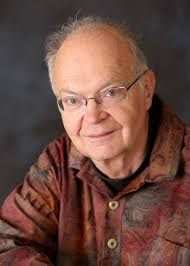
\includegraphics[width=.6\textwidth]{knuth}
\caption{پروفسور دونالد کنوث }
\end{minipage}
\hfill
\begin{minipage}{.4\textwidth}
\centering
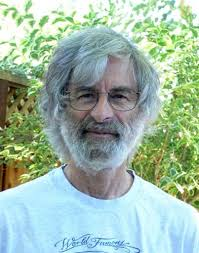
\includegraphics[width=.6\textwidth]{lamport}
\caption{پروفسور لزلی لمپورت }
\end{minipage}
\end{figure}
طی سال‌های بعد از آن کنوث و افراد دیگری روی آن کار کردند. اما با توجه به سطح
پایین بودن دستورات آن، کار با آن کمی سخت بود. در اوایل دهۀ 1980 میلادی 
لِزلی لمپورت\LTRfootnote{Leslie Lamport}
یک مجموعه از ماکروهای \lr{\TeX} را جمع‌آوری و به نام \lr{\LaTeX}\footnote{تلفظ این
کلمه «لِیتِک» یا «لاتِک» است.} ارائه کرد. این نگارش دستوراتی را در اختیار کاربران قرار می‌داد
که بیشتر نیازهای آن‌ها را برآورد می‌کرد و لذا استفاده از آن مشابه استفاده از زبان‌های
برنامه‌نویسی سطح بالا، برای سطح وسیع‌تری از کاربران قابل استفاده می‌کرد، بدون آن که
نیاز به یادگیری مفاهیم زیادی داشته باشند. طی سالیان بعدی، \lr{\TeX} به سطح وسیعی
پیشرفت کرد و به تبع آن توسط بسیاری افراد، ناشرین و مجلات علمی مورد استفاده 
قرار گرفت و این پیشرفت و استفاده با سرعت بالای هنوز نیز ادامه دارد. 
در خصوص تاریخچه به همین مقدار بسنده می‌کنیم و خواننده علاقه‌مند را به مرجع \cite{TeXHis} ارجاع می‌دهیم.

\section{چرا \lr{\TeX} یا \lr{\LaTeX}؟}
اگر نشریه یا کتابی آماده کرده باشید و قصد چاپ آن را داشته باشید چه می‌کنید؟ بدیهی
است ابتدا باید متن شما (که به فرض دست‌نویس است) حروف‌چینی شود و سپس برای 
چاپ فرستاده شود. البته در بیشتر موارد، حروف‌چینی با تایپ هم معنی در نظر گرفته 
می‌شود که از نظر حرفه‌ای این دو تفاوت بسیار دارند. کارِ حروف‌چین، یک کار تخصصی است
که بسته به کاربرد متن، مشخص می‌کند مثلاً در هر خط از کتاب، چند کلمه یا کاراکتر باشد
و در هر صفحه چند خط قرار بگیرد و یا اشکال کتاب در کجا قرار بگیرند و هر خط در 
کدام قسمت شکسته شود و بسیاری موارد دیگر. کیفیت کار حروف‌چین در محصول نهایی
بسیار موثر است و گاهی یک کتاب بسیار مفید به دلیل کیفیت پایین حروف‌چینی
که باعث ناخرسندی خواننده از بسیاری جهات می‌شود، با اقبال خوبی مواجه نمی‌شود.

لذا برای ایجاد یک محصول خوب و استاندارد، لازم است از حروف‌چینی استفاده
شود که تبحر لازم در این حرفه را داشته باشد و با پیشرفت‌های این رشته آشنا باشد
و از آخرین تکنیک‌های حروف‌چینی در کار خود استفاده کند. با توجه به کامپیوتری
شدن کارها، حروف‌چینی نیز به کامپیوترها منتقل شده است و برنامه‌های بسیاری
برای حروف‌چینی ارائه شده است. بحث اصلی این است که ما از کدام حروف‌چین
کامپیوتری برای کار خود استفاده کنیم؟  اولین جواب و شاید تنها جواب اکثر کاربران
به این پرسش نرم‌افزار \lr{Word} از مجموعۀ \lr{Microsoft Office} است. اما اولین نکته اینجاست
که \lr{Word} اصلاً یک نرم‌افزار حروف‌چین نیست بلکه یک واژه‌پرداز یا 
\lr{Word Processor} است (مراجع \cite{Word,beuty,Art} را ببینید). یک واژه‌پرداز، محیطی در اختیار شما قرار 
می‌دهد تا مشابه یک دستگاه تایپ، شما متن خود را وارد کنید. هرچند در نگارش‌های
جدید واژه‌پردازها امکانات زیادی اضافه شده است ولی هنوز هم این نرم‌افزارها را
به عنوان حروف‌چین نمی‌شناسند. لذا استفاده از یک نرم‌افزار واژه‌پرداز برای حروف‌چینی
مصداق بردن «بوریا باف» به «کارگاه حریر» در مثل فارسی است.

البته افراد حرفه‌ای در صنعت چاپ احتمالاً به نرم‌افزار \lr{InDesign} اشاره می‌کنند
که البته یک نرم‌افزار حروف‌چین است، اما علاوه بر قیمت بالای این محصول و تخصصی
بودن استفاده از آن، به اعتقاد بسیاری از کارشناسان حروف‌چینی، محصول تولید شده
توسط \lr{\TeX}  کیفیت بالاتری نسبت به محصول \lr{InDesign} دارد. در ذکر کیفیت\lr{\TeX}  
همین بس که در تبلیغات  \lr{InDesign}  در جایی گفته شده است که این نرم‌افزار از الگوریتم‌های استفاده شده در \lr{\TeX}   استفاده می‌کند. 

چند مورد از مزایای \lr{\TeX} \ را می‌توان به شرح زیر بیان کرد:
\begin{itemize}
\item اولاً تِک مجانی و متن-باز است و نسخه‌های مجانی آن روی تمام سیستم‌عامل‌ها موجود است. از
جمله توزیع‌های مجانی تِک می‌توان به \lr{\TeX{}Live}، \lr{Mik\TeX} اشاره کرد.
برای دیدن لیست کامل از توزیع‌های تِک  و مقایسۀ قابلیت‌های آن‌ها به مرجع~\cite{Latex} مراجعه کنید.
\item تِک هم پایدار و هم قابل انعطاف است. اهمیت موضوع پایداری برای افرادی که متونی
را در \lr{Word} آماده کرده‌اند کاملاً قابل فهم است. زیرا ممکن نیست با مشکلات عدم پایداری
آن که به نوعی برخورد نکرده باشند. این عدم پایداری در \lr{Word} به حدی است که
طنزهای بسیاری نیز برای آن بیان شده است، مثل این که احتمال قاطی کردن \lr{Word}
با میزان اهمیت متن تایپ شده نسبت مستقیم و با زمان باقیمانده شخص 
برای کامل کردن متن، نسبت عکس دارد! از دید قابلیت انعطاف همین بس که کاربر حتی
می‌تواند فاصله بین کاراکترها را کم یا زیاد کند. 
\item امکان فرمول‌نویسی با استفاده از تِک، اولاً نسبتاً ساده است و ثانیاً خروجی
ایجاد شده بسیار شکیل است. حتی فرمول‌های بسیار پیچیده را به راحتی می‌توان
در تِک با استفاده از دستوراتی نوشت و کیفیت خروجی فرمول به حدی است که به جرأت
می‌توان گفت، همتا ندارد.
\item امکان گرفتن خروجی \lr{PDF} مستقیم از آن وجود دارد و خروجی \lr{PDF}
تولید شده، هم دارای کیفیت بسیار بالایی است و هم حجم بسیار کمی نسبت به سایر نرم‌افزارها
دارد. میزان این کیفیت به نوعی است که برخی برای تولید تصاویر  برداری با کیفیت
از تِک استفاده می‌کنند. نرم‌افزارهای گرافیکی وجود دارند که نیازهای کاربر را از طریق یک رابط
گرافیکی دریافت می‌کند و آن را تبدیل به فایل مناسب حروف‌چینی با تِک کرده و سپس محصول نهایی
را با استفاده از تک تولید می‌کند. امکانات و بسته‌های گرافیکی موجود برای تِک بسیار کامل 
است. 
%برای نمونه بارکد تولید شده در انتهای همین مقاله، با استفاده از یکی از این بسته‌ها 
%ایجاد شده است. تاکید می‌کنم که این بارکد مربعی مستقیماً در همین مقاله تولید شده و اینطور نیست 
%که در نرم‌افزار دیگری تولید شود و در این مقاله درج شود.
\item قابل حمل است به این معنی که یک فایل آماده شده با تِک را برای هر فردی بفرستید،
اولاً آن شخص صرفنظر از این که از کدام توزیع تِک و در کدام سیستم‌عامل 
استفاده می‌کند، می‌تواند آن را استفاده کرده و با خروجی دقیقاً یکسان با آنچه شما دریافت می‌کنید
آن را بسازد. این خاصیت وقتی با حجم کم فایل‌های آن (زیرا فایل‌های آن فایل‌های متنی ساده است)
 نیز در نظر گرفته شود، یک امکان
منحصر به فرد برای انجام پژوهش‌های مشترک بین افرادی که از راه دور ارتباط دارند، فراهم
می‌کند.
\item بسیار پویا  است و به راحتی قابل توسیع است. همین امر با در نظر گرفتن متن-باز
بودن آن امکانی را فراهم کرده است که افراد بتوانند بر مبنای آن بسته‌هایی را برای
کارهای خود آماده و ضمن استفاده، در اختیار سایر کاربران قرار دهند. لذا خیلی دور از ذهن
نیست کاری را که شما قصد انجام آن را دارید، قبلاً در بسته‌ای آماده شده باشد و شما
به راحتی بتوانید از آن استفاده کنید. مثلاً فرض کنید بخواهید نوتهای موسیقی خود را
در تِک تایپ کنید. با یک جستجوی ساده در موتورهای جستجو به مرجع~\cite{Music}
می‌رسید. و یا اگر تصمیم دارید بخش‌های از قرآن و یا ترجمه آن  را در متن خود داشته باشید 
مرجع~\cite{quran} را خواهید یافت. 
\item امکان استفاده از آن در حروف‌چینی زبان‌های مختلف وجود دارد، حتی زبان‌هایی
کاملاً متفاوت با انگلیسی نظیر زبان‌های فارسی و عربی که از راست به چپ نوشته می‌شوند
و زبان‌های پیچیده‌ای نظیر چینی~\cite{Art}.
\item متون تهیه شده در تِک بسیار ساختاریافته است و لذا به راحتی و بدون نیاز به 
ویرایش مجدد، می‌توان قالب آن را عوض کرد. این مزیت، یکی از اصلی‌ترین دلایلی است
که مجلات از این نرم‌افزار استفاده می‌کنند زیرا به راحتی با دریافت فایل اصلی تِک مقاله
و با اندک تغییراتی می‌توانند آن را در فرمت مجلۀ خود آماده کنند. البته بسیاری نیز با توجه
به سادگی کار، فرمت را که در قالب یک فایل آماده شده است در اختیار نویسنده قرار می‌دهند
تا مقاله را با آن فرمت تهیه کند. متون آماده شده با تِک را به ظرفی پر از مایع تشبیه
می‌کنند که به راحتی می‌توان به ریختن مایع در یک قالب، آن مایع را به شکل آن 
 قالب درآورد.
 \item استفاده از تِک برای حروف‌چینی از طریق خط فرمان است و هیچ رابط گرافیکی
 خاصی نیاز ندارد. البته، محیط‌های مختلف برای نوشتن و حروف‌چینی آن موجود و برخی
 مجانی و برخی غیرمجانی در دسترس است ولی آن‌ها نیز از دستورات خط فرمانی
 تِک برای کار خود استفاده می‌کنند. از این محیط‌ها می‌توان به 
 \lr{Winedit}\LTRfootnote{\url{http://www.winedt.com/}}
 و \lr{TeXMaker}\LTRfootnote{\url{http://www.xm1math.net/texmaker/}}
 اشاره کرد. لیست محیط‌های مربوط به تِک و مقایسۀ آن‌ها 
 را می‌توانید در مرجع~\cite{Editors} ببینید.
 \item انجام بسیاری از کارهای حروف‌چینی  نظیر شماره گذاری
 فصل‌ها و بخش و \linebreak زیربخش‌ها، فرمول‌ها، اشکال و جداول به صورت اتوماتیک است.
همچنین استفاده از یک سیستم ارجاع 
 مبتنی بر برچسب جهت به روزرسانی خودکار ارجاعات و تهیه خودکار مواردی چون
 فهرست مطالب، فهرست اشکال و نمایه برای متون که انجام آن به صورت معمول هم 
 زمان‌بر است و هم با اشتباهات متعددی روبرو می‌شود را به صورت خودکار انجام می‌دهد.
 ضمن این که به دلیل انجام خودکار
 این کارها، در صورت انجام تغییراتی در متن، تمام این موارد قابل انجام به صورت مجدد جهت
 به روزرسانی است. فقط تصور کنید که در ویرایش کتاب شما، فقط یک فصل به یکی از
 فصول اولیه کتاب اضافه شده است. با این تغییر مختصر باید اولاً شماره تمام فصول بعدی
 تغییر کند و ثانیاً در ارجاعات به این فصول نیز این تغییرات اعمال شود که حتی فکر کردن 
 به انجام دستی  آن باعث سردرد می‌شود!
 \item در متون، برخی قسمت‌ها نظیر جداول و اشکال را اشیاء شناور می‌نامند به این معنی
 که حروف‌چین می‌تواند آن را در قسمت‌های مختلفی بیاورد و مکان ثابتی برای آن‌ها وجود ندارد.
 تِک از یک الگوریتم مناسب جهت جایابی این اشیاء شناور استفاده می‌کند به صورتی که
 نتیجه بسیار مناسب است. همزمان این امکان را به نویسنده می‌دهد که اگر برای شیء شناوری،
 محل خاصی مد نظر دارد، بتواند آن را نیز اعمال کند.
   \end{itemize}
   
   در اینجا به بیان همین مزایا بسنده می‌کنیم. لازم است در کنار مزایا، به موارد و افرادی 
   نیز اشاره    کنیم که  استفاده از تِک توصیه نمی‌شود. 
   \begin{itemize}
   \item  اگر زمان کافی برای یادگیری تِک ندارید، مطمئناً این انتخاب مناسبی
   برای شما نیست. زیرا ممکن است با نرم‌افزارهایی نظیر \lr{Word} حتی با فرض
   عدم آشنایی بتوانید متنی را آماده‌سازی کنید ولی این اتفاق در تِک نمی‌افتد. لذا در شروع
   کار لازم است زمان کافی برای یادگیری حداقل اصول آن صرف کنید. هرچند به شما
   اطمینان می‌دهیم چندین برابر وقتی را که در اینجا صرف می‌کنید در تهیه متن خود
   با این سیستم صرفه‌جویی خواهید کرد.
   \item اگر محیط‌های \lr{WYSIWYG}\LTRfootnote{\lr{What You See Is What You Get}}
   نظیر \lr{Word} را می‌پسندید. در استفاده از تِک شما باید فایل منبعی را آماده کنید
   که یک فایل متنی اسکی یا یونیکد است. سپس این فایل را به حروف‌چین تِک 
   می‌دهید تا متن حروف‌چینی شده را آماده کرده و به شما تحویل دهد. لذا امکان دیدن همزمان
   نتیجه در زمان تایپ متن ورودی وجود ندارد. البته اخیرا پروژه‌ای برای این 
   منظور به نام   \lr{LyX}\LTRfootnote{http://www.lyx.org/}
   معرفی شده است که سعی در اضافه کردن این قابلیت 
   به  تِک  دارد ولی پیش‌بینی می‌شود با توجه به مشکلاتی که این قابلیت ایجاد می‌کند،
   استفاده از آن خیلی جذاب نباشد.
   \item هیچ زمینه‌ای در برنامه‌نویسی کامپیوتر ندارید. در نهایت تِک یک زبان برنامه‌نویسی
   حروف‌چینی است و لذا در روند حروف‌چینی، ممکن است با خطاهای متعددی 
روبرو شوید که لازم است مشابه رفع خطاهای گرامری\LTRfootnote{Syntax error}
یک برنامه، آن‌ها را پیدا  و رفع کنید.   یادآوری می‌شود که در نهایت تِک یک زبان برنامه‌نویسی است.
   \end{itemize}

\section{ساختار فایل و روش استفاده}   
 برای استفاه از حروف‌چین تِک، متن خام باید در یک ویرایشگر تایپ شده و 
 سپس فایل حاصل (که پسوند آن \lr{.tex} است)
 به برنامۀ حروفچین
 با استفاده از خط فرمان داده شود. ویرایشگرهایی وجود دارند که امکان وارد کردن 
 متن خام
 و به طور همزمان، امکان دادن فایل به موتور \lr{\TeX} و نشان دادن نتیجۀ حروف‌چینی را دارند. 
 اما تمام آن‌ها بر مبنای همان دستورات خط فرمان عمل می‌کنند و هیچکدام به تنهایی و بدون
 دسترسی به یک موتور \lr{\TeX} نمی‌توانند خروجی تولید کنند. البته هیچ وابستگی بین
 ویرایشگر و فایل تولید شده توسط آن وجود ندارد و یک فایل توسط هر کدام می‌تواند 
 تولید یا ویرایش شود یا فایل ایجاد شده توسط  یک ویرایشگر، در دیگری تغییر یابد.
 
    برای حروفچینی فایل، می‌توان از طریق خط فرمان به صورت زیر عمل کرد. در ویندوز
    وارد \lr{Command Prompt } شوید و به محل قرار گرفتن فایل مربوطه (همان فایل با پیوند \lr{.tex}) بروید. بسته به کاربرد خود  و شکل خروجی مورد نظر 
    یکی از دستورات زیر را بزنید تا فایل خروجی مربوطه ایجاد شود. به جای \lr{filename}  نام فایل با پسوند \lr{.tex} گذاشته شود. 


    \begin{center}
    \begin{tabular}{|lr|}
    \hline
    \lr{latex filename} &  برای خروجی \lr{.dvi} با فایل ورودی انگلیسی \\
     \lr{pdflatex filename} & برای خروجی \lr{.pdf} با فایل ورودی انگلیسی\\ 
     \lr{xelatex filename} & برای خروجی \lr{.pdf} با فایل ورودی فارسی یا  انگلیسی \\ 
    \hline
    \end{tabular}
    \end{center}

    \textcolor{red}{توجه:} دقت کنید که نام فایل یا فولدرهایی که فایل در آن قرار دارد فارسی
    نباشد یا بین نام آن‌ها فاصله وجود نداشته باشد. در صورت عدم رعایت این موضوع، در برخی
    مواقع اجرا با مشکل روبرو می‌شود.

    فایل آماده شده خام، شامل دستوراتی است که قسمت‌های مختلف متن نظیر عنوان فصل و بخش
    و سایر موارد را مشخص می‌کند. اگر این دستورات درست استفاده نشده باشند، حروفچین در زمان
    حروفچینی خطا می‌دهد که پیام خطا شامل شماره خطی است که در آن خطا اتفاق افتاده است.
    لذا، در این موارد باید مشابه خطاگیری از یک برنامۀ کامپیوتری، نسبت به رفع خطا اقدام کرد.
    توجه کنید که موتور تِک در صورت وجود خطا ممکن است متن را به صورتی به غیر از آنچه مورد نظر است حروفچینی
    کند و اگر تعداد خطاها زیاد باشد ممکن است قسمت یا کل متن را حروفچینی نکند و خروجی
    نداشته باشد یا خروجی حاصل ناقص باشد.

 
 در اینجا به نمونه‌ای کوچک از فایل خام حروف‌چینی و نتیجۀ حروف‌چینی می‌آوریم. 
 برای فایل حاوی متن زیر (سمت راست)
 خروجی شکل روبرویش ایجاد می‌شود.
 \bigpar
 \begin{minipage}{0.4\textwidth}
 \latin \small
 \begin{verbatim}
\documentclass[12pt]{article}
\begin{document}
\title{Title of paper}
\author{First LastName}
\maketitle
\section{Section title}
some text here and formula 
$$\sum_{i=1}^\infty 
\frac{e^x}{1+\frac{1}{x}}.$$
\subsection{sub-section}
And here ...
\section{Section two}
Something
\end{document}
 \end{verbatim}
 \end{minipage}
 \begin{minipage}{0.6\textwidth}
 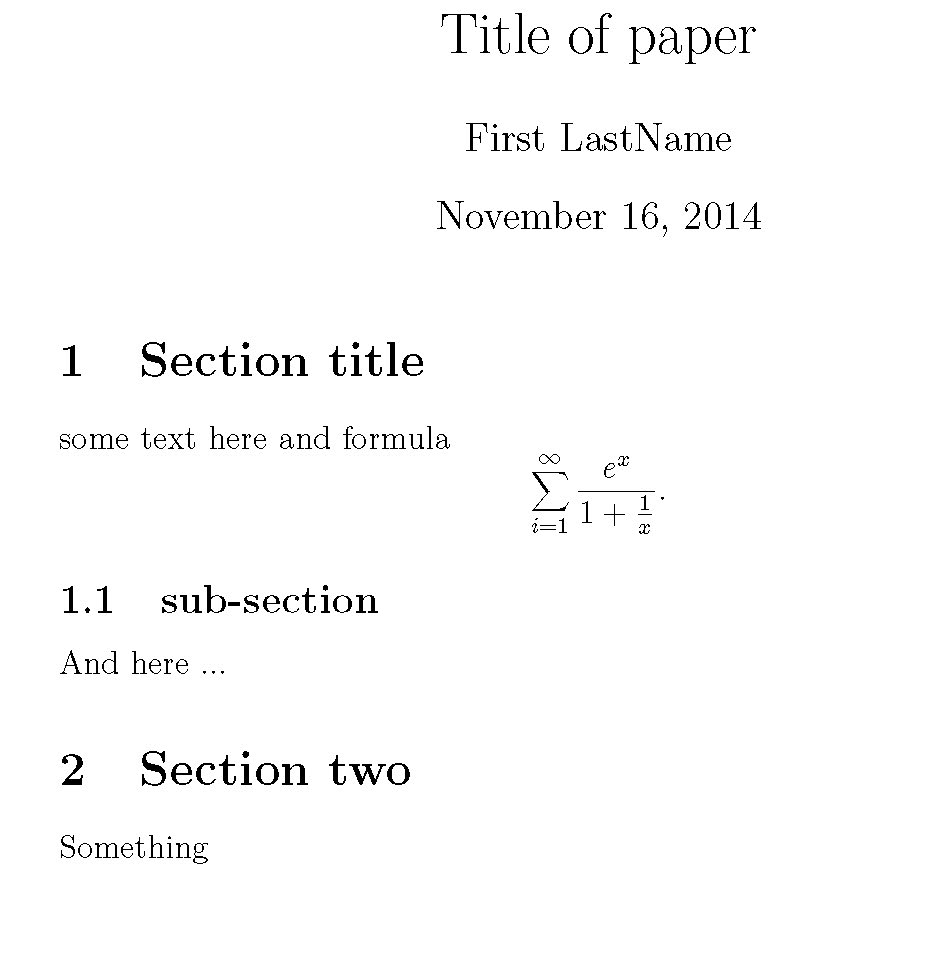
\includegraphics[width=0.9\textwidth]{test-crop}
 \end{minipage}
 
\section{منابع آموزشی و فایل‌های نمونه}
جهت یادگیری دستورات و شکل استفاده از تِک، منابع زیادی وجود دارد که اکثراً به رایگان
در دسترس هستند. 
     اگر نوشتن پایان‌نامه/رساله اولین تجربه شما از کار با لاتک است، توصیه می‌شود که یک‌بار، 
     کتاب \hbox{«%
    \href{http://opac.nlai.ir/opac-prod/bibliographic/4728642}{%
    مقدمه‌ای بر زی‌پرشین و ریاضی‌نویسی در \lr{\LaTeX}}»}%
    \cite{razavianAmintoosiTayebi}
    و یا کتاب «%
    \href{http://www.tug.ctan.org/tex-archive/info/lshort/persian/lshort.pdf}{مقدمه‌ای نه چندان کوتاه بر \lr{\LaTeXe}}»%
    \cite{Omidali1387Lshort}\footnote{این کتاب ترجمه‌ای از \cite{lshort} است.}
        را مطالعه کنید. کتاب اول، کتاب بسیار کاملی است که خیلی از نیازهای شما را در ارتباط با حروف‌چینی فارسی/لاتین، مقاله، 
        پایان‌نامه/رساله\cite{AmintoosiHSUThesis}، پوستر\cite{xebaposter} و یا حتی  ارائه\cite{beamer} برطرف می‌کند.
        درکتاب دوم، می‌توانید برخی مطالب جزئی‌تر را که در کتاب اول اشاره نشده است بیابید. مطالعه \cite{lamport} جنبه‌های بیشتری از لاتِک را برایتان مشهود 
        می‌سازد و اگر می‌خواهید که در زبان تِک به یک متخصص تبدیل شود \cite{knuth:texbook} را مطالعه نمایید. در آخر از آنجایی که برای حروفچینی 
        پارسی باید که بسته‌ٔ \Verb+xepersian+ (و به صورت ضمنی بستهٔ \Verb+bidi+) را بکار برد لذا توصیه اکید به مطالعه \cite{bidi,xepersian}
        در ادامه منابع قبلی است. 
    اگر هم تمایل دارید کمی با تاریخچه زی‌پرشین آشنا شوید مقالات\cite{Xepersian-IMS-1391,Xepersian-IMS-1392,newamintoosi} را نگاه کنید. 

    علاوه بر این‌ها می‌توانید در لینک زیر برخی از این منابع و همچنین اسلایدهایی برای آموزش که توسط دکتر فرشی گردآمده است را مشاهده نمایید.

\centerline{\url{http://cs.yazd.ac.ir/farshi/LaTeX/LaTeX.html}}

    به خاطر داشته باشید که یادگیری تِک نیاز به زمان و حوصله دارد اما مطمئن باشید ارزش آن را دارد.
 % chapter 1
    \chapter{راهنمای استفاده از کلاس \lr{\protect\ttfamily \lowercase{thesis-qom}}}
    \section{مقدمه}
    حروف‌چینی پایان‌نامه/رساله یکی از موارد پرکاربرد استفاده از تِک/لاتِک در بین دانشجویان و شاید نقطه شروع آشنایی ایشان با این سیستم بی‌نظیر است. 
    خوب از آنجایی که نگارش باید به زبان پارسی باشد، یکی از بهترین انتخاب‌ها، زی‌پرشین است. علاوه بر پایان‌نامه/رساله امکان حروفچینی نامه، 
    مقاله، پوستر و حتی ارائه نیز با زی‌پرشین مقدور است. از طرفی، یک  پایان‌نامه/رساله،  احتیاج به تنظیمات زیادی از نظر صفحه‌آرایی  دارد 
    تا مطابق با نظر تحصیلات تکمیلی موسسه مطبوع گردد و همین ممکن است برای
    یک کاربر مبتدی، کمی مشکل باشد. گرچه غالب کاربران تا کنون بارها بارها از نرم‌افزار مایکروسافت ورد استفاده کرده‌اند لکن به جرات 
    می‌توان گفت که بیشتر آنان از زمره کاربران عادی این نرم‌افزار هستند و توانایی حروفچینی حرفه‌ای با آن را ندارند. به همین سبب برخی موسسات 
    اقدام به تهیه یک قالب آماده ورد برای دانشجویان می‌نمایند ولی متاسفانه این قالب معمولاً برای یکی از نسخه‌های ورد تهیه می‌شود و در دیگر نسخه 
    به درستی عمل ننموده و دانشجویان را به دردسر می‌اندازد؛ از طرف دیگر لاتک چنین محدودیتی ندارد و کاربران به راحتی می‌توانند از کیفیت خروجی 
    مطمئن بوده و بدون هیچ نگرانی، تنها به متن خود بپردازند. 
    به همین دلایل، برای راحتی کار کاربر، کلاس حاضر با نام 
     \LRE{\Verb!thesis-qom!}
     برای حروف‌چینی پروژه‌ها، پایان‌نامه‌ها و رساله‌های دانشگاه قم با استفاده از نرم‌افزار زی‌پرشین،  آماده شده است. این فایل به 
    گونه‌ای طراحی شده است که کلیه خواسته‌های مورد نیاز  مدیریت تحصیلات تکمیلی دانشگاه قم را برآورده می‌کند. همچنین حروف‌چینی بسیاری
    از قسمت‌های آن، به طور خودکار انجام می‌شود.

    کلیه فایل‌های لازم برای حروف‌چینی با کلاس گفته شده، داخل پوشه‌ای به نام
     \LRE{\Verb!thesis-qom!}
      قرار داده شده است. توجه داشته باشید که برای استفاده از این کلاس باید فونت‌هایی که در پوشه \Verb+fonts+ قرار دارد روی 
        روی سیستم شما نصب شده باشد. این پوشه شامل فونت‌های ذیل است:‌
        \begin{enumerate*}
            \item \Verb+Yas+
            \item \LR{\Verb+XB Niloofar+}
             \item \Verb+IranNastaliq+
            \item \Verb+IRLotus+
            \item \LR{\Verb+XB Zar+}
            \item \LR{\Verb+XB Titre+}
        \end{enumerate*}
        
    \section{این همه فایل؟!}\label{sec2}
    از آنجایی که یک پایان‌نامه یا رساله، یک نوشته بلند محسوب می‌شود، لذا اگر همه تنظیمات و مطالب پایان‌نامه را داخل یک فایل قرار بدهیم، باعث شلوغی
    و سردرگمی می‌شود. به همین خاطر، قسمت‌های مختلف پایان‌نامه یا رساله  داخل فایل‌های جداگانه قرار گرفته است. مثلاً تنظیمات  کلاس داخل فایل
    \LRE{\Verb!settings.tex!}، 
    مطالب فصل اول، داخل \linebreak
    \Verb!chapter1!
    و ... قرار داده شده است. نکته مهمی که در اینجا وجود دارد این است که از بین این  فایل‌ها، فقط فایل 
    \LRE{\Verb!thesis.tex!}
    قابل اجرا است. یعنی بعد از تغییر فایل‌های دیگر، برای دیدن نتیجه تغییرات، باید این فایل را اجرا کرد. بقیه فایل‌ها به این فایل، کمک می‌کنند تا بتوانیم خروجی کار را ببینیم. اگر به فایل 
    \LRE{\Verb!thesis.tex!}
    دقت کنید، متوجه می‌شوید که قسمت‌های مختلف پایان‌نامه، توسط دستورهایی مانند 
    \Verb!input!
    و
    \Verb!include!
    به فایل اصلی، یعنی 
    \LRE{\Verb!thesis.tex!}
    معرفی شده‌اند. بنابراین، فایلی که همیشه با آن سروکار داریم، فایل 
    \LRE{\Verb!thesis.tex!}
    است.
    در این فایل، فرض شده است که پایان‌نامه/رساله، شامل چند فصل و پیوست است. با این حال، اگر
      پایان‌نامه/رساله، به فصول یا پیوست‌های بیشتر نیاز دارد، باید خودتان فصل‌های بیشتر را به این فایل، اضافه کنید. این کار، بسیار ساده است. فرض کنید بخواهید یک فصل دیگر هم به پایان‌نامه، اضافه کنید. برای این کار، کافی است یک فایل با نام 
    \Verb!chapterN!  --\lr{N} شماره فصل بعدی--
    و با پسوند 
    \Verb!.tex!
    بسازید و آن را داخل پوشه 
    \LRE{\Verb!thesis-qom!}
    قرار دهید و سپس این فایل را با دستور 
    \Verb!\include{chapterN}!
    داخل فایل
    \LRE{\Verb!thesis.tex!}
    و بعد از آخرین دستور
    \Verb!\include!
    و قبل از \Verb+\appendix+ قرار دهید. حال اگر می‌خواهید یک پیوست دیگر بیفزایید باید آن را پس از آخرین \Verb!\include! 
    که بعد از \Verb+\appendix+ آمده است قرار دهید. 

    \section{از کجا شروع کنم؟}
    قبل از هر چیز، بدیهی است که باید یک توزیع تِک مناسب مانند 
    \Verb!Live TeX!
    و یک ویرایش‌گر تِک مانند
    \Verb!Texmaker!
    را روی سیستم خود نصب کنید.  نسخه بهینه شده \Verb!Texmaker!  را می‌توانید  از سایت 
     \href{http://www.parsilatex.com}{پارسی‌لاتک}%
    \LTRfootnote{\url{http://www.parsilatex.com}}
     و \Verb!Live TeX!  را هم می‌توانید از 
     \href{http://www.tug.org/texlive}{سایت رسمی آن}%
    \LTRfootnote{\url{http://www.tug.org/texlive}}
     دانلود کنید و یا آن را از طریق 
     \href{http://parsilatex.com/site/?p=185}{فروشگاه سایت پارسی‌لاتک}%
    \LTRfootnote{\url{http://parsilatex.com/site/?p=185}}
     به همراه مجموعه‌ای غنی از مثال، کتاب و فیلم آموزشی تهیه نمایید. برای توضیحات بیشتر به پیوست~\ref{chap:installation} مراجعه نمایید. 
     
    در مرحله بعد، سعی کنید که  یک پشتیبان از پوشه 
    \LRE{\Verb!thesis-qom!}
     بگیرید و آن را در یک جایی از هارددیسک سیستم خود ذخیره کنید تا در صورت خراب کردن فایل‌هایی که در حال حاضر، با آن‌ها کار می‌کنید، همه چیز را از 
     دست ندهید. البته برای گرفتن یک پشتیبان روی فضای اینترنت می‌توانید از 
     \href{https://www.dropbox.com/}{دراپ‌باکس}%
    \LTRfootnote{\url{https://www.dropbox.com/}}
      و یا 
      \href{https://github.com}{گیت‌هاب}%
    \LTRfootnote{\url{https://github.com}}
       استفاده نماید تا هر زمان که به کامپیوتر خود 
     دسترسی نداشتید نیز بتوانید براحتی از طریق وب، فایل‌هایتان را بررسی نمایید؛‌ البته پشیتبان‌گیری روی اینترنت محدود به گزینه‌ها نبوده و دانشجویان 
     می‌توانند  خدمات دیگری اعم از رایگان یا پولی را بکار برند. 
     
     \subsection{ مشخصات پایان‌نامه/رساله}
    بعد از موارد گفته شده، فایل 
    \LRE{\Verb!settings.tex!}
    را باز کنید و مشخصات پایان‌نامه خود مثل نام، نام خانوادگی، عنوان پایان‌نامه و ... را جایگزین مشخصات موجود در فایل
     کنید. هر چند که شاید نیاز به ایجاد یک فایل مجزا برای اینکار نبود لکن همانطور که در بخش~\hbox{\ref{sec2}} شرح داده شد با اینکار، سعی داریم که فایل 
     اصلی، \Verb!thesis.tex!، تنها نشان دهندهٔ ساختار محتوایی پایان‌نامه/رساله شما باشد. 
     در  فایل \Verb!settings.tex! دستوری به نام \Verb+\thesisdetails+ وجود دارد که تمامی پارامترهای لازم از طریق این دستور تنظیم می‌شود. 
     دقت داشته باشید که نیازی نیست 
    نگران چینش این مشخصات در فایل پی‌دی‌اف خروجی باشید. فایل     \LRE{\Verb!thesis-qom.cls!}
    همه این کارها را به طور خودکار برای شما انجام می‌دهد. در ضمن، موقع تغییر دادن دستورهای داخل فایل
    \LRE{\Verb!settings.tex!}
     کاملاً  دقت کنید. این دستورها، خیلی حساس هستند و ممکن است با یک تغییر کوچک، موقع اجرا، خطا بگیرید. برای دیدن خروجی کار، فایل 
     را     \Verb!Save!،     (نه     \Verb!As Save!)    کنید و بعد به فایل 
    \LRE{\Verb!thesis.tex!}
    برگشته و آن را اجرا کنید.
    
    همانطوری که تاکنون با نگاه به فایل \LRE{\Verb!settings.tex!} متوجه شده‌اید، تمامی تنظیمات لازمه درون دستوری به نام \Verb+\thesisdetails+ 
    قرار دارد و برای مقداردهی کافی است مقدار مطلوب پس از علامت \Verb+=+ که بعد از نام فیلد مورد نظر آمده است درج گردد؛‌ توجه نمایید که 
    اگر مقدار فیلد مطلوب بیش از یک خط به خود اختصاص می‌دهد این مقدار باید بین آکولاد باز و بسته محصور گردد و یا اینکه محتویات مطلوب 
    در فایلی جداگانه نوشته شده و سپس در جلوی آن فیلد با دستورات \Verb+\input+  و یا \Verb+\include+ وارد گردد. 
    جداکننده بین فیلدها کاراکتر کامای لاتین است؛ دقت نماید که به اشتباه کاراکتر ویرگول فارسی را بکار نبرید. 

    فیلدها در دو دسته فارسی و لاتین تعریف شده‌اند که نام خود فیلد گویا بوده و نیاز به توضیح اضافی ندارد. فیلدهای فارسی تعریف‌شده 
    در جدول~\ref{tab:persianfields} آمده است. تنها نکته‌ای که باید در نظر داشته باشید این است که در فرم دفاع در جلوی نام اساتید مرتبه 
    علمی آن‌ها نیز نوشته خواهد شد لذا برای مشخص نمودن مرتبه علمی استاد مورد نظر باید مرتبه ایشان را داخل پرانتز جلوی نام ایشان بنویسید، همانند 
    \fbox{دکتر اکبر طیبی (دانشیار)}. 
    نکته فوق شامل «نماینده تحصیلات تکمیلی» نیز می‌گردد. فیلدهای لاتین نیز در جدول~\ref{tab:latinfields} آمده است. دقت نمایید که تمامی 
    فیلدهای لاتین با حروف کوچک نگاشته شده‌اند و تغییر حالت هر یک از حروف این فیلدها سبب بروز خطا می‌گردد. 
    
\begin{table}[htb]
\caption{فیلدهای فارسی قالب پایان‌نامه/رساله تعریف شده در دستور \lr{\textbackslash{}thesisdetails}}
\label{tab:persianfields}
\smallskip
\hrule\hrule
\begin{multicols*}{3}
    \begin{enumerate}
        \item نام و نام‌خانوادگی
        \item شماره دانشجویی
        \item عنوان
        \item دانشکده
        \item گروه
        \item رشته
        \item گرایش
        \item تاریخ اتمام
        \item تاریخ دفاع
        \item تعداد واحد
        \item نمره
        \item نمره به حروف
        \item درجه
        \item استاد راهنمای اول
        \item استاد راهنمای دوم
        \item استاد مشاور اول 
        \item استاد مشاور دوم
        \item داور داخلی اول
        \item داور داخلی دوم
        \item داور خارجی اول
        \item داور خارجی دوم
        \item {\footnotesize  نماینده تحصیلات تکمیلی}
        \item تقدیم به
        \item نیایش
        \item سپاسگزاری
        \item چکیده
        \item کلمات کلیدی
    \end{enumerate}
\end{multicols*}
\hrule
\end{table}

\begin{table}[htb]
\caption{فیلدهای لاتین قالب پایان‌نامه/رساله تعریف شده در دستور \lr{\textbackslash{}thesisdetails}}
\label{tab:latinfields}
\begin{latin}
\ttfamily
\smallskip
\hrule\hrule
\LTRmulticolcolumns
\begin{multicols*}{3}
    \begin{enumerate}
        \item author
        \item title
        \item faculty
        \item department
        \item submission~date
        \item first~supervisor
        \item second~supervisor
        \item first~advisor
        \item second~advisor
        \item abstract
        \item keywords
    \end{enumerate}
\end{multicols*}
\end{latin}
\hrule
\end{table}

    برای راحتی بیشتر،     فایل     \LRE{\Verb!thesis-qom.cls!}
        طوری طراحی شده است که کافی است فقط  یک‌بار مشخصات پایان‌نامه/رساله  را وارد کنید. هر جای دیگر که لازم به درج این مشخصات باشد، 
        این مشخصات به طور خودکار درج می‌شود. از جمله ویژگی‌های این کلاس این است که هیچکدام از فیلدها اجباری نبوده و در صورتی که 
        تعریف نشده باشند در صورت نیاز جای آن‌ها خالی گذاشته می‌شود. 
        
        اگر مایل بودید، می‌توانید تنظیمات موجود را در قالب اصلی تغییر دهید لکن توجه داشته باشید که اگر کاربر مبتدی هستید 
        و یا با ساختار فایل‌های      \Verb!cls!     آشنایی ندارید، به هیچ وجه به این فایل، یعنی فایل     \LRE{\Verb!thesis-qom.cls!}
        دست نزنید.

    \subsection{گزینه‌های کلاس}
    نکته دیگری که باید به آن توجه کنید این است که برای حروفچینی، رساله دکتری به صورت پیش‌فرض انتخاب شده است، لذا اگر 
    تمایل به حروفچینی پایان‌نامه و یا پروژه کارشناسی را دارید باید به ترتیب گزینه‌های \Verb+ms+ و یا \Verb+bs+ را به 
    کلاس     \LR{\Verb!thesis-qom.cls!} ارسال دارید. 
    با این کار، تنظیمات مربوطه به طور خودکار  اعمال می‌شود و جای هیچگونه نگرانی وجود ندارد.    
    
    گزینه‌های تعریف شده در قالب فعلی به شرح جدول~\ref{tab:options} است. 

\newcounter{tabline}
    
    \begin{table}[hbtp]
    \caption{گزینه‌های قالب پایان‌نامه/رساله}
    \label{tab:options}
    \smallskip
    \begin{tabularx}{\textwidth}%
    {@{\hskip 1pt}>{\ifnum\thetabline=0\else\thetabline\fi\refstepcounter{tabline}}c@{\hskip 1pt}>{\bgroup\ttfamily}c<{\egroup}X}
    \hline
      {\footnotesize ردیف} & \rl{ گزینه}  & \multicolumn{1}{c}{توضیحات} \\ \hline
        & bs & 
        تنظیمات لازم برای پروژه کارشناسی صورت خواهد گرفت؛ ضمناً صفحات «تأییده داوران» و «اصالت پایان‌نامه/رساله» حروفچینی نخواهد شد.\\
        & ms & تنظیمات لازم برای پایان‌نامه کارشناسی‌ارشد صورت خواهد گرفت. \\
        & phd & 
         تنظیمات لازم برای رساله دکتری صورت خواهد گرفت؛ به طور پیش‌فرض این گزینه فعال است لذا نیازی به درج این گزینه نیست. \\
        & index &
         تنظیمات لازم برای درج نمایه در پایان‌نامه/رساله؛ توجه داشته باشید در صورت بکار بردن این گزینه برای کامپایل سند باید از سوئیچ 
         \LR{\Verb+--shell-escape+} نیز استفاده نمود.\\
        & final &
         با فعال نمودن این گزینه صفحات «تأییده داوران» و «اصالت پایان‌نامه/رساله»، «تقدیم به»، «نیایش» و صفحه «سپاسگزاری» حروفچینی خواهند شد.\\
        & print & 
        به طور پیش‌فرض لینک‌ها در حروفچینی رنگی بوده و ضمناً در بخش مراجع شماره‌ صفحاتی که به آن مرجع اشاره شده است درج می‌گردد که مناسب نسخه 
        چاپی پایان‌نامه/رساله نمی‌باشند. لذا با بکار بردن این گزینه می‌توانید نسخه نهایی را برای چاپ آماده نمایید.  \\ 
        \hline
    \end{tabularx}
    \end{table}
    
    سندی که در حال حاضر در دست شما است با گزینه‌های \Verb+index+ و \Verb+final+ حروفچینی شده است به عبارت دیگر 
    اولین خط فایل {\ttfamily \jobname.tex} برابر است با: 
    
    \hfill\LR{\Verb+\documentclass[index, final]{thesis-qom}+}
    
    \subsection{محیط‌های قضیه‌مانند }        
    در قالب پایان‌نامه/رساله دانشگاه قم، تعدادی محیط قضیه‌مانند به شرح زیر تعریف شده است که کاربران می‌توانند به فراخور نیاز آن‌ها را 
    بکار برند. برای آشنایی با این محیط‌ها جدول~\ref{tab:theoremenvs} را مشاهده نمایید. 
    \begin{table}[!htbp]
        \centering
        \caption{محیط‌های قضیه‌مانند تعریف شده در کلاس پایان‌نامه/رساله دانشگاه قم}
        \label{tab:theoremenvs}
        \begin{tabular}{>{\bgroup\ttfamily}c<{\egroup}c>{\bgroup\latin}c<{\egroup}}
                \rl{محیط} & توضیح & \rl{سبک نگارش} \\
                \hline
            definition  & تعریف & definition \\
            example & مثال & '' \\
            theorem & قضیه & plain \\
            lemma    & لم & '' \\
            proposition & گزاره & '' \\
            corollary & نتیجه & '' \\
            remark & ملاحظه & remark \\
            point & نکته & '' \\
        \end{tabular}
    \end{table}
    
    چند نمونه از کاربرد این محیط‌ها را در بخش~\ref{sec:shortexp} می‌تواند مشاهده نمایید؛ در این بخش محیط‌های تعریف، قضیه و مثال 
    استفاده شده‌ است.
    
     \subsection{امکانات دیگر قالب پایان‌نامه/رساله دانشگاه قم}
     همانطوری که از دوران آغازین تحصیل علم آموخته‌ایم در زبان پارسی، صفر باید به صورت توخالی نگاشته شود. 
     متاسفانه با همه گیر شدن کامپیوتر و طراحی فونت‌های متعدد توسط افرادی که به این نکته توجه نداشتند و یا اینکه اساسا فونت‌ها را 
     برای زبان‌هایی مانند عربی،‌ کردی و یا ترکی ایجاد نموده بودند از این نکته غافل شده و امروزه شاید شما بیش چند فونت معدود نیابید 
     که این نکته را دارا باشد که از آن جمله می‌توان به قلم‌های \lr{Yas}  و \lr{PGaramond} اشاره نمود. متاسفانه فونت‌های مذکور 
     قلم مناسبی برای حروفچینی متن اصلی پایان‌نامه/رساله ندارند. از آنجایی که متن پایان‌نامه/رساله یک متن علمی است انتظار می‌رود که 
     نویسنده آن این نکته را مد نظر داشته باشد لکن با توجه به اینکه تغییر دائم فونت توسط کاربر کمی صعب به نظر می‌رسد، 
     کلاس \LR{\Verb+thesis-qom+}  این کار را به صورت خودکار برای کاربر انجام می‌دهد و نیاز به اعمال دستی این نکته نمی‌باشد. 
     فقط باید متذکر گردید که فونت مورد استفاده فونت یاس است لذا انتظار می‌رود که فونت مذکور روی سیستم کاربر نصب باشد. 
     
     نکته دیگر که به صورت خودکار در این قالب در نظر گرفته می‌شود شمارش تعداد کلمات موجود در چکیده فارسی/انگلیسی سند است. 
     اگر این تعداد از ۳۰۰ کلمه تجاوز نماید بسته به اینکه این اتفاق در چکیده فارسی یا لاتین رخ داده است یکی از پیام‌های زیر را دریافت 
     خواهید داشت. تصاویر \ref{fig:abswarfa}  و \ref{fig:abswaren} را مشاهده نمایید. در اعلان خطاهای مورد نظر \lr{NNN} 
     تعداد کلمات بکار رفته در چکیده را نشان می‌دهد که بیشتر از ۳۰۰ کلمه شده است. 
     
     \begin{figure}[!hbtp]
        \caption{پیام خطای تجاوز چکیده از حد مجاز در حالت فارسی.}   
        \label{fig:abswarfa}   
        \centerline{\color{red}\bfseries\zarfont "متن چکیده نباید بیش از ۳۰۰ کاراکتر باشد؛‌ لطفاً آن را ویرایش نمایید.``}
        \centerline{\color{gray}\bfseries\zarfont در حال حاضر متن چکیدهٔ شما حاوی \lr{NNN} کلمه است!}
        
             
       \caption{پیام خطای تجاوز چکیده از حد مجاز در حالت لاتین.}        
        \label{fig:abswaren} 
        \medskip
    \begin{latin}
        \centerline{\color{red}\bfseries ``The Abstract cannot contain more than 300 words."}
        \centerline{\color{gray}\bfseries This one includes NNN words! Please modify it.}%
    \end{latin}    
     \end{figure}
     
    از جمله دیگر امکانات می‌توان به درج خودکار نمادها که جلوتر معرفی گردید و نیز حروفچینی خودکار واژه‌نامه‌های فارسی و انگلیسی اشاره داشت 
    که کمی بعد با آن‌ها در فصل~\ref{chap:bibindex} آشنا خواهید شد. 
    \subsection{ساختار کلی سند اصلی}
    با رعایت نکاتی که در فوق مطرح گردید ساختار کلی سند اصلی پایان‌نامه/رساله‌ شما باید به صورت زیر باشد.

\begin{latin}    
\begin{lstlisting}[title=\rl{ساختار کلی سند اصلی}, escapechar={|},]
\documentclass[options]{thesis-qom}
    
\usepackage{pkg1}
\usepackage{pkg2}
|$\vdots$|
% |\rl{فایل زیر حاوی فیلدهای پایان‌نامه/رساله که در دستور \lr{\textbackslash{}thesisdetails} تعریف شده است.}|    
\thesisdetails{
نام و نام‌خانوادگی=ندا ایزدیان,
شماره دانشجویی=۹۶۱۲۱۴۱۰۱۸,
عنوان=بررسی کلاس منیفلدهای لندزبرگی تعمیم‌یافته, %فرمت نگارش پایان‌نامه/رساله دانشگاه قم,
دانشکده=علوم پایه,
گروه=ریاضیات, 
رشته=ریاضی محض,
گرایش=هندسه,
استاد راهنمای اوّل=دکتر اکبر طیبی (دانشیار),
استاد راهنمای دوّم=دکتر حسن نجومی(دانشیار),
استاد مشاور اوّل=دکتر مرتضی میرزایی(استادیار),
استاد مشاور دوّم=دکتر علیرضا توکلی(استادیار),
نماینده تحصیلات تکمیلی=دکتر سیداحمد فقیهی  (دانشیار),
تاریخ اتمام=مهر ۱۳۹۶,
تاریخ دفاع=۱۳۹۶/۰۷/۱۴,
تعداد واحد=6, 
نمره=19.25, 
نمره به حروف=نوزده و بیست و پنج صدم, 
درجه=عالی, % گزینه‌های ممکن عالی، بسیار خوب، خوب، قابل قبول'
داور داخلی اوّل=دکتر نسرین صادق‌زاده (استادیار),
داور داخلی دوّم=استاد داور داخلی دوّم(استاد),
داور خارجی اوّل=استاد داور خارجی اوّل(استاد),
داور خارجی دوّم=استاد داور خارجی دوّم(استاد),
author=Neda Izadian, 
title=On the class of generalized Landsberg Manifolds, % University of Qom's Thesis Style, 
faculty=Science,
department=Mathematics, 
major=Pure Mathematics, 
field=Geometry, 
submission date=November 2017, 
first supervisor=Dr. Akbar Tayebi,
%second supervisor=Dr. Hasan Nojumi,
first advisor=Dr. Morteza Mirzaie,
%second advisor=Dr. Alireza Tavakoli,
abstract=%----------------------------------------------------------------------------------------
%در این قسمت چکیده انگلیسی آورده می‌شود.
%----------------------------------------------------------------------------------------

In $2000$, Bejancu-Farran introduced the class of generalized Landsberg  manifolds which contains the class of Landsberg manifolds. In this thesis, we prove three global results for generalized Landsberg manifolds. First, we show that every compact generalized Landsberg manifold is a Landsberg manifold. Then we prove that every complete generalized landsberg manifold with relatively isotropic landsberg curvature reduces to a Landsberg manifold. Finally, we show that every generalized Landsberg manifold with vanishing Douglas curvature satisfies $ H=0 $. 
,
keywords={Landsberg Manifold, Riemannian Curvature, H-Curvature, Berwald Metric.  },%{Thesis, Style, XePersian, }, 
تقدیم به={ %بجای اینکه در این نقطه مطالب را ذکر کنید می‌توانید توضیحات را درون یک فایل نوشته و آن را در اینجا \input نمایید مانند شیوه‌ای که برای abstract در دو خط بالاتر بکار رفت. 
تقدیم به همسر و فرزندان عزیزم

که در این راه مرا تحمل نموده و صبورانه همراهی کردند 

\begin{traditionalpoem}
          تا ذوق درونم خبری می‌دهد از دوست &  از طعنه دشمن به خدا گر خبرستم \\
          می‌خواستمت پیشکشی لایق خدمت  &   جان نیک حقیرست ندانم چه فرستم \\
\end{traditionalpoem}
}, % پایان تقدیم به 
نیایش={\zarfont
منّت خدای را عز و جل که طاعتش موجب قربتست و به شکر اندرش مزید نعمت، هر نفسی که فرو می رود ممدّ حیاتست و چون بر می آید مفرّح ذات. 
پس در هر نفسی دو نعمت موجودست و بر هر نعمتی شکری واجب.
\begin{traditionalpoem}
از دست و زبان که برآید & کز عهده شکرش به در آید
\end{traditionalpoem}
اِعملوا آلَ داودَ شکراً وَ قلیلٌ مِن عبادیَ الشکور 

\begin{traditionalpoem}
بنده همان به که ز تقصیر خویش &  عذر به درگاه خدای آورد \\
ورنه سزاوار خداوندیش  &  کس نتواند که به جای آورد\\
\end{traditionalpoem}

باران رحمت بی حسابش همه را رسیده و خوان نعمت بی‌دریغش همه جا کشیده پرده ناموس بندگان به گناه فاحش ندرد و وظیفه روزی به خطای منکر نبرد

\begin{traditionalpoem}
ای کریمی که از خزانه غیب & گبر و ترسا وظیفه خور داری\\
دوستان را کجا کنی محروم & تو که با دشمن این نظر داری\\
\end{traditionalpoem}

}, % پایان نیایش
سپاسگزاری={\zarfont 
با تشکر از معاونت محترم آموزشی که موجبات فراهم آمدن چنین بسته‌ای را ممکن ساختند. 

اگر تلاش‌های شبانه‌روزی و بی‌شائبهٔ وفا خلیقی (توسعه دهنده بستهٔ فاخر زی‌پرشین) در طی ۱۲ سال اخیر نبود، امروز آماده‌سازی 
متون علمی پارسی در لاتک قطعاً با مشقات زیادی همراه بوده و شاید در نظر برخی تا حدی ناممکن می‌نمود. لذا قدردان زحمات بی‌منّت او 
بوده و برای او در هر کجای گیتی که باشد آرزوی سلامتی داریم. این استایل از ایده‌های دکتر خیلقی بهره‌های بسیار برده است. 

همچنین لازم است از کاربران گروه پارسی‌لاتک نیز تشکر به عمل آوریم که در طی سالیان اخیر با پاسخگویی به سوالات کاربران راهگشای ایشان بوده‌اند. 
},  % پایان سپاسگزاری
چکیده=%\input{abs},
{\zarfont  
چکیده شامل خلاصه‌ای از هدف یا مسأله پژوهش، روش شناسی، نتایج و تفسیر می‌‌شود که خواننده با مطالعه آن از محتوای
پژوهش آگاه می‌شود. در چکیده از اشاره به تاریخچه، تفصیل اقوال، توصیف تکنیک‌ها، فصل‌بندی، ذکر منابع و آوردن فرمول‌ها،
نمودارها و جداول پرهیز می‌شود. متن چکیده حداکثر باید 300 کلمه باشد و در یک صفحه و در یک بند (پاراگراف) نگاشته شود.
همچنین واژگان کلیدی در یک سطر جداگانه درج می شود و تعداد آن بین 5 تا 8 کلمه می‌باشد.},
کلمات کلیدی={چکیده،‌ پایان‌نامه، رساله، شیوه‌نامه، زی‌پرشین},
} % end of \thesisdetails macro
 
 
 
 \newcommand{\wi}[1]{\index{#1}#1}
\newcommand{\wil}[1]{\index{\lr{#1}}\lr{#1}}

% تنظیمات ذیل برای درج کد لاتک در سند استفاده شده است. 
\lstset{% general command to set parameter(s)
    float=htbp,
    language=[LaTeX]tex,
    numbers=left, 
    numberstyle=\tiny\yasfont,
    frame=single,
    frameround=fttt,
    gobble=0,
    breaklines=true,
%    escapechar={|},
    aboveskip=2\medskipamount,
}

 

\begin{document}

\chapter*{پیشگفتار}

    دانشجویان تحصيلات تکمیلی برای ارائه پایان‌نامه/رساله خود ملزم به رعایت چارچوب کلی تعیین شده توسط معاونت پژوهشی موسسه/دانشگاه مطبوع خود 
    هستند. با توجه به اینکه رعایت دقیق این نکات توسط دانشجو امری زمان‌بر بوده و در نهایت هم مستلزم بررسی توسط ناظر شکلی تحصیلات تکمیلی و 
    کتابخانه دانشگاه است، عموماً با توجه به حجم کار و گستردگی آن مستندات تحویلی یک دست نبوده و دقیقاً مطابق با آنچه در قانون آمده است 
    نخواهد شد و مسئولین امر برای اینکه دانشجو به مشقت نیفتند معمولاً با دیده اغماض به این اشکالات نگریسته و از آن در می‌گذرند. 
    به همین سبب در برخی مؤسسات اقدام به آماده‌سازی قالبی از پیش‌آماده می‌نمایند تا به میزان زیادی از این اشکالات ناخواسته جلوگیری گردد. 
    
    هر چند که امروزه نرم‌افزار مایکروسافت ورد انتخاب اول کاربران برای حروفچینی اسناد است لکن این نرم‌افزار یک حروفچین نبوده و تنها یک ویرایشگر 
    پیشرفته متن است. نکتهٔ فوق و دیگر اینکه دانشجویان علوم پایه و بعضاً فنی مهندسی بخصوص رشته‌های ریاضی، فیزیک، برق و کامپیوتر در اسناد 
    خود با فرمول‌های ریاضی سر و کار دارند بهترین انتخاب را سیستم حروفچینی لاتک \lr{(\LaTeX{})} می‌یابند --
    گرچه در گروه ریاضی و فیزیک دانشگاه قم دانشجویان ملزم به آماده‌سازی پایان‌نامه خود با لاتک هستند--. 
    دانشجویان با وجود لاتک و یک قالب آماده، 
     دیگر هیچ نگرانی برای حروفچینی متن و رعایت دستورالعمل نگارشی دانشگاه ندارند و تمامی موارد 
    --همچون اندازه و نوع قلم متن و عناوین، اندازه حاشیه‌ها، صفحات 
    آغازین، سبک منابع و مآخذ و \ldots \hspace{2mm}-- به صورت خودکار توسط قالب آماده شده اعمال می‌گردد. 
    از این نقطه به بعد دانشجویان، دیگر تنها کافی است که روی متحوای کار خود تمرکز نمایند. 
    اگرچه ممکن است برای برخی دانشجویان یادگیری دستورات لاتک در بدو امر کمی مشکل باشد، امّا به تدریج با دستورات آن آشنا خواهند شد و 
    در ادامه در خواهند یافت که چقدر حروفچینی با لاتک آسان و دلنشین است. 
    
    کلاس پایان‌نامه/رساله دانشگاه قم سعی نموده با نگاهی به تمامی کلاس‌های موجود، کلاسی را فراهم آورد که کار کردن با آن برای دانشجویان بسیار ساده باشد و به نظر 
    نیز چنین است. در این کلاس هیچ فیلد اجباری وجود ندارد و تمامی مقادیر به صورت پیش‌فرض مقداردهی می‌شوند و در صورتی که کاربر 
    مقداری برای فیلدهای متناظر تعریف نماید از آن فیلد‌ها استفاده خواهد شد. از جمله دیگر مزایای این کلاس، تمرکز اصلی دانشجو بر محتوای سند 
    است و لازم نیست که دستورات ویژه یا نکات خاصی را در نگارش خود رعایت نماید و کلاس سعی نموده است که تمامی کارهای لازمه را به صورت 
    خودکار انجام دهد. 
    
    قطعاً این قالب بدون نقص نبوده و در صورت دریافت بازخورد از سمت کاربران، توسعه‌دهندگان خود را متعهد به اصلاح آن می‌دانند. ضمناً در صورت 
    نیازهای جدید کاربران نیز تا آنجایی که معقول باشد بر خود وظیفه می‌دانند که آن‌ها را نیز بمرور زمان و در حد امکان برآورده نمایند. امید است 
    این قالب وظیفه دانشجویان را در آماده‌سازی پایان‌نامه/رساله تسهیل نماید و ذهن آنان را معطوف به متن اصلی خود نماید. 
 % |\rl{پیشگفتار؛ در صورت نیاز}|

\tableofcontents % |\rl{فهرست مطالب}|
\listoffigures % |\rl{فهرست تصاویر}|
\listoftables % |\rl{فهرست جداول}|
\listofsymbols % |\rl{فهرست نمادها}|
\lstlistoflistings % |\rl{فهرست برنامه‌ها}|
        
\include{chapters/chap1} % chapter 1
\include{chapters/chap1} % chapter 1
|$\vdots$|        
\appendix %|\rl{پیوست‌}|
\include{chapters/app1} % appendix 1
\include{chapters/app2} % appendix 2
|$\vdots$|
\end{document} 
\end{lstlisting}
\end{latin}
    همانطور که مشاهده می‌نمایید در این ساختار هیچ صحبتی از نمایه،‌ واژه‌نامه‌های فارسی و انگلیسی و نیز منابع و مآخذ بمیان نیامده است و 
    همانگونه که جلوتر توضیح داده می‌شود این‌ها به صورت خودکار از روی فایل‌هایی که مشخص شده است تولید می‌گردد. البته نمایه به هیچ 
    فایل خاصی وابسته نیست و تماماً در متن پایان‌نامه/رساله نگاشته می‌شود.
        
    \section{مطالب پایان‌نامه/رساله را چطور بنویسم؟}
    \subsection{نوشتن فصل‌ها}
    همان‌طور که در بخش \ref{sec2} گفته شد، برای جلوگیری از شلوغی و سردرگمی کاربر در هنگام حروف‌چینی، قسمت‌های مختلف پایان‌نامه/رساله 
    از جمله فصل‌ها، در فایل‌های جداگانه‌ای قرار داده شده‌اند. 
    بنابراین، اگر می‌خواهید مثلاً مطالب فصل ۱ را تایپ کنید، باید فایل‌های 
    \LRE{\Verb!thesis.tex!}
    و
    \Verb!chapter1!
    را باز کنید و محتویات داخل فایل 
    \Verb!chapter1!
    را پاک کرده و مطالب خود را تایپ کنید. توجه کنید که همان‌طور که قبلاً هم گفته شد، تنها فایل قابل اجرا، فایل 
    \LRE{\Verb!thesis.tex!}
    است. لذا برای دیدن حاصل (خروجی) فایل خود، باید فایل  
    \Verb!chapter1!
    را 
    \Verb!Save!
    کرده و سپس فایل 
    \LRE{\Verb!thesis.tex!}
    را اجرا کنید. یک نکته بدیهی که در اینجا وجود دارد، این است که لازم نیست که فصل‌های پایان‌نامه/رساله را به ترتیب تایپ کنید. می‌توانید ابتدا 
    مطالب فصل ۳ را تایپ کنید و سپس مطالب فصل ۱ را تایپ کنید. 

    نکته بسیار مهمی که در اینجا باید گفته شود این است که سیستم \lr{\TeX}، محتویات یک فایل تِک را به ترتیب پردازش می‌کند. به عنوان مثال، 
    اگر فایلی، دارای ۴ خط دستور باشد، ابتدا خط ۱، بعد خط ۲، بعد خط ۳ و در آخر، خط ۴ پردازش می‌شود. بنابراین، اگر مثلاً مشغول تایپ 
    مطالب فصل ۳ هستید، بهتر است     که دو دستور 
    \Verb!\include{chapter1}!     و     \Verb!\include{chapter2}!     را در فایل     \LR{\Verb!thesis.tex!}،
    غیرفعال\footnote{    برای غیرفعال کردن یک دستور، کافی است پشت آن، یک علامت    \%     بگذارید.    }
     کنید. زیرا در غیر این صورت، ابتدا مطالب فصل ۱ و ۲ پردازش شده (که به درد ما نمی‌خورد؛ چون ما می‌خواهیم خروجی فصل ۳ را ببینیم) 
     و سپس مطالب فصل ۳ پردازش می‌شود و این کار باعث طولانی شدن زمان اجرا می‌شود. زیرا هر چقدر حجم فایل اجرا شده، بیشتر باشد، 
     زمان بیشتری هم برای اجرای آن، صرف می‌شود.
     
    \subsection{مراجع}
    مرجع \cite{Omidali82phdThesis} یک نمونه پروژه دکترا و مرجع \cite{Vahedi87} یک نمونه مقاله مجله فارسی است.
    مرجع \cite{Amintoosi87afzayesh}  یک نمونه  مقاله کنفرانس فارسی و
    مرجع \cite{vahid90} یک نمونه کتاب فارسی است. مرجع \cite{Khalighi07MscThesis} یک نمونه پروژه کارشناسی ارشد انگلیسی و
    \cite{Khalighi87xepersian} هم یک نمونه متفرقه  می‌باشند.

    مرجع \cite{Gonzalez02book} یک نمونه کتاب لاتین است که از آنجا که دارای فیلد \lr{authorfa} است، 
    نام نویسندگان آن در استایل‌های \lr{asa-fa}، \lr{plainnat-fa} و \lr{chicago-fa} به فارسی دیده می‌شود\cite{Amintoosi1394persianbib}. 
    مرجع \cite{Baker02limits} مقاله انگلیسی است که معادل فارسی نام نویسندگان آن ذکر نشده بوده است.

    برای تولید مراجع باید از دستور \lr{bibtex} استفاده کنید. در صورتی که بخواهید مراجع فارسی قبل از
    مراجع انگلیسی بیایند، باید به جای دستور \lr{bibtex thesis} از دستور زیر استفاده کنید:

    \begin{latin}
    \LR{\Verb+bibtex8 -W -c cp1256fa thesis+}
    \end{latin}
    
    
    \subsection{واژه‌نامه فارسی به انگلیسی و برعکس}
    برای وارد کردن واژه‌نامه فارسی به انگلیسی و برعکس، چنانچه کاربر مبتدی هستید، بهتر است مانند روش بکار رفته در فایل‌های 
    \Verb!dicfa2en!
    و
    \Verb!dicen2fa!
    عمل کنید. امّا چنانچه کاربر پیشرفته هستید، بهتر است از بسته
    \Verb!glossaries!
    استفاده کنید. راهنمای این بسته را می‌توانید به راحتی و با یک جستجوی ساده در اینترنت پیدا کنید.
    \subsection{نمایه}
    برای وارد کردن نمایه، باید از 
    \Verb!xindy!
    استفاده کنید. زیرا 
    \Verb!MakeIndex!
    با حروف «گ»، «چ»، «پ»، «ژ» و «ک» مشکل دارد و ترتیب الفبایی این حروف را رعایت نمی‌کند. همچنین، فاصله بین هر گروه از کلمات در 
    \Verb!MakeIndex!،
    به درستی رعایت نمی‌شود که باعث زشت شدن حروف‌چینی این قسمت می‌شود. راهنمای چگونگی کار با 
    \Verb!xindy! 
    را می‌توانید در تالار گفتگوی پارسی‌لاتک، پیدا کنید.

    دستور مربوطه به صورت زیر است:

    \label{xindy}
    \begin{latin}
%    \footnotesize
%    xindy -L persian-variant1 -C utf8 -M numeric-sort -M latex -M latex-loc-fmts -M texindy %.idx
    \begin{Verbatim}
xindy -L persian-variant1 -C utf8 -M texindy thesis.idx
    \end{Verbatim}
    \end{latin}
    ممکن است بکار بردن دستورات فوق کمی برایتان مشکل باشد لذا بدین منظور تنها کافی است که کلاس را با گزینهٔ \Verb+index+ فراخوانی نمایید 
    و برای کامپایل آن از سوئیچ \LR{\Verb+--shell-escape+} استفاده نمایید؛ در این صورت تمامی این کار به صورت خودکار در تنها در یک گام پردازش 
    انجام خواهد شد لکن در فرض استفاده از زیندی،  فایل اصلی --در اینجا \Verb+thesis.tex+-- باید یکمرتبه دیگر کامپایل شود.
    
    \subsection{ نمادها}
    به منظور تولید «فهرست نمادها»، کلاس \LR{\Verb+thesis-qom+} تسهیلاتی را برایتان فراهم می‌آورد. 
    برای درج یک نماد در این فهرست،‌ در اولین نقطه‌ای که یک نماد را معرفی می‌نمایید با کمک دستور زیر، نماد و توصیف آن را شرح دهید:
    
    \hfill\LR{\Verb+\addsymbol{name}{symbol}{description}+}
    
    با کمک \Verb+name+ بعدها می‌توان به نماد تعریف شده و توصیف آن دسترسی داشت. \Verb+symbol+ 
    همان نمادی خواهد بود که در سند     می‌خواهیم نشان دهیم و \Verb+description+ نیز توصیف نماد است. 
    پس از دستور فوق سه دستور دیگر به شرح زیر تعریف می‌شوند که پس از این در هر کجای سند که به نماد تعریف شده نیازی بود بسته به 
    کاربرد می‌توان یکی از دستورات ذیل را بکار برد: 
    \begin{itemize}
        \item \Verb+\sym{name}+ این دستور سبب حروفچینی توصیف و نماد به صورت \linebreak
        \LR{\Verb+description (symbol)+} می‌گردد. 
        \item \Verb+\syms{name}+ سبب حروفچینی نماد تعریف شده می‌گردد؛ یعنی همان  \Verb+symbol+. 
        \item \Verb+\syml{name}+ سبب حروفچینی توصیف نماد تعریف شده می‌گردد؛ یعنی همان \linebreak\Verb+description+. 
    \end{itemize}
    
    با اینکار نماد و توصیف آن به صورت خودکار به لیست نمادها افزوده خواهد شد 
    سپس برای نمایش «فهرست نمادها»  دستور \Verb+\listofsymbols+ را بکار برید. 

    \subsection{مثالی کوتاه}
    \label{sec:shortexp}
    % در اولین مکانی که نمادی را تعریف می‌نمایید می‌تواند با دستور \addsymbol آن را به فهرست نمادها اضافه نمایید. 
    \addsymbol{real}{$\mathbb{R}$}{مجموعه اعداد حقیقی}
    \addsymbol{img}{$\mathbb{C}$}{مجموعه اعداد موهومی}
    \addsymbol{nat}{$\mathbb{N}$}{مجموعه اعداد طبیعی}
    \addsymbol{cpu}{\lr{CPU}}{\lr{Central Processing Unit}}
    % پس از  تعاریف فوق به ازای هر نماد سه دستور  \sym و  \syms و  \syml تعریف می‌گردند که با نام تعریف شده نماد قابل استفاده هستند. 
    % دستور اول نام تفصیلی نماد را که در جلوی آن خود نماد درون پرانتز آمده است را حروفچینی می‌نماید و دستور دوم تنها خود نماد و دستور 
    % سوم هم  توضیح نماد را نمایش خواهد داد. 
        
    در ادامه، برای فهم بیشتر مطالب، چند تعریف، قضیه و مثال آورده شده است.  سپس با نمادهای\index{نماد} 
    \sym{real}،‌ \sym{img} و  \syml{nat} (\syms{nat})
    از نماد 
    \sym{cpu} نیز استفاده خواهیم کرد!

    
    \begin{definition}
    مجموعه همه ارزیابی‌های  (پیوسته)  روی $(X,\tau)$، دامنه توانی احتمالی
    \index{دامنه توانی احتمالی}
    $ X $
    نامیده می‌شود.
    \end{definition}
    \begin{theorem}[باناخ-آلااغلو]
    \index{قضیه باناخ-آلااغلو}
    اگر $ V $ یک همسایگی $ 0 $ در فضای برداری 
    \index{فضای!برداری}
     توپولوژیکی $ X $ باشد و 
    \begin{equation}\label{eq1}
    K=\left\lbrace \Lambda \in X^{*}:|\Lambda x|\leqslant 1 ; \ \forall x\in V\right\rbrace,
    \end{equation}
    آنگاه $ K $،  ضعیف*-فشرده است که در آن، $ X^{*} $ دوگان
    \index{فضای!دوگان}
     فضای برداری توپولوژیکی $ X $ است به ‌طوری که عناصر آن،  تابعی‌های 
    خطی پیوسته
    \index{تابعی خطی پیوسته}
     روی $X$ هستند.
    \end{theorem}
    تساوی \eqref{eq1} یکی از مهم‌ترین تساوی‌ها در آنالیز تابعی است که در ادامه، به وفور از آن استفاده می‌شود.
    \begin{example}
    برای هر فضای مرتب، گردایه 
    $$U:=\left\lbrace U\in O: U=\uparrow U\right\rbrace $$
    از مجموعه‌های بالایی باز، یک توپولوژی تعریف می‌کند که از توپولوژی اصلی، درشت‌تر  است.
    \end{example}
    حال تساوی 
    \begin{equation}\label{eq2}
    \sum_{n=1}^{+\infty} 3^{n}x+70x=\int_{1}^{n}8nx+\exp{(2nx)}
    \end{equation}
    را در نظر بگیرید. با مقایسه تساوی \eqref{eq2} با تساوی \eqref{eq1} می‌توان نتیجه گرفت که ...
    
        


    \section{چاپ فایل پی‌دی‌اف}
    فایل پی‌دی‌اف حاصل از این بسته، مطمئناً مطابق با آیین‌نامه نگارش پایان‌نامه دانشگاه قم
    است و این امر توسط کارشناسان مرکز تحصیلات تکمیلی دانشگاه قم تایید شده است.
    امّا چاپ فایل پی‌دی‌اف حاصل نیز باید به صورتی باشد که در خروجی تغییراتی داده نشود و نسخۀ
    چاپ شده نیز مطابق با دستورالعمل باشد. 

     مشکل اصلی این است که برخی تنظیمات پرینتر، باعث ایجاد تغییرات در محصول نهایی می‌شود.
      حتی تغییر پرینتر نیز گاهی آن‌ها را عوض می‌کند. 
     نکته‌ای که مشکل را حل می‌کند این است که، اولا حتما مطئن شوید 
     که اندازه کاغذ انتخابی در موقع پرینت، همان \lr{A4} باشد و ثانیا تمام گزینه‌های مربوط 
     به \lr{Page Handling}  را غیرفعال کنید. نمونه به صورت زیر است:

     {\centerline{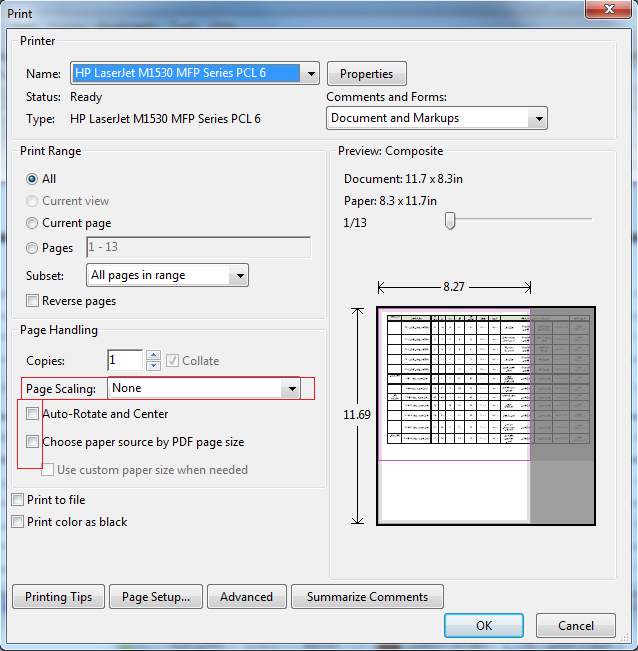
\includegraphics[width=0.6\textwidth]{Print-PDF}}}
     
    دقت کنید که بسته به پرینتر شما ممکن است موارد دیگری نظیر \lr{shrinking}  و غیره نیز 
    موجود باشد که باید همه غیر فعال شوند.
    با این ترتیب، مطمئناً حاشیه‌ها مطابق حاشیه‌ها در فایل پی‌دی‌اف خواهد بود.
    \section{اگر سوالی داشتیم، از چه کسی  بپرسیم؟}
    برای پرسیدن سوال‌های خود در مورد حروف‌چینی با زی‌پرشین،  می‌توانید به سایت‌های 
     \hbox{\href{http://qa.parsilatex.com}{ پرسش و پاسخ پارسی‌لاتک}}%
    \LTRfootnote{\url{http://qa.parsilatex.com}} 
    و یا 
    \hbox{\href{https://tex.stackexchange.com/questions}{\lr{Stack Exchange}}}%
    \LTRfootnote{\url{https://tex.stackexchange.com/questions}}
    مراجعه کنید. شما هم می‌توانید روزی به سوال‌های دیگران در این سایت جواب بدهید.
        

    \section{جمع‌بندی}
    در این فصل به بیان مقدمات نحوه استفاده از قالب پایان‌نامه/رساله دانشگاه قم پرداخته شد. 
    گرچه که مطالعه کامل این راهنما مقداری وقت شما را خواهد گرفت، اما مطمئن باشید از اتلاف وقت شما در ادامه کارتان تا حد زیادی جلوگیری خواهد کرد. 
    در نوشتن متن حاضر سعی شده است بیشتر مواردی که عموماً دانشجوان با آن مواجه هستند - و با نگاه ویژه به نیازهای دانشجویان ریاضی - ذکر شود. 
    در ادامه نوشتار نمونه مواردی از درج تصویر، نمودار، کد برنامه، الگوریتم، توضیحات، منابع، فرمول، تعریف، قضیه، مثال و جدول آمده است. 
    توصیه می‌شود یک کپی از کل فایل‌های این قالب را جداگانه از نسخه پایان‌نامه/رساله خود نگهداری نمایید تا در صورت نیاز بتوانید مراجعه فرمایید. 
    همچنین توصیه اکید داریم که رفع خطاهایی که احتمالاً با آن مواجه می‌شوید را به آخر موکول نفرمایید و به محض برخورد با خطا، آن را اشکال‌زدایی نموده و 
    خطا را برطرف فرمایید.
 % chapter 2
% !TEX TS-program = XeLaTeX
% !TeX root=main.tex

\chapter{آشنایی سریع با برخی دستورات لاتک}\label{Chap:chapter2}

در این فصل ویژگی‌های مهم و پرکاربرد زی‌پرشین و لاتک معرفی می‌شود. برای راهنمایی بیشتر و به کاربردن ویژگی‌های پیشرفته‌تر به راهنمای زی‌پرشین 
و راهنمای لاتک مراجعه کنید. 

\section{بندها و زیرنویس ها}
هر جایی از نوشتهٔ خود، اگر می خواهید به سر سطر بروید و یک پاراگراف تازه را آغاز کنید، باید یک خط را خالی بگذارید.

حالا که یک بند تازه آغاز شده است، یک زیرنویس انگلیسی%
\LTRfootnote{English Footnote!}
 هم می نویسیم!
\section{فرمول‌های ریاضی}\label{formula}

اینجا هم یک فرمول می آوریم که شماره دارد:
\begin{equation}\label{eq:yek}
A=\frac{c}{d}+\frac{q^2}{\sin(\omega t)+\Omega_{12}}
\end{equation}

%\RTLcolumnfootnotes

در لاتک می توان به کمک فرمان 
\Verb+\label{}+
به هر فرمول یک نام نسبت داد. در فرمول بالا نام \lr{eq:yek} را برایش گذاشته‌ایم (پروندهٔ \lr{tex} همراه با این مثال را ببینید). این نام ما را قادر می‌کند که بعداً بتوانیم با فرمان
\Verb+\ref{eq:yek}+
به آن فرمول با شماره ارجاع دهیم. یعنی بنویسیم فرمول \ref{eq:yek}. 
لاتک خودش شمارهٔ این فرمول‌ها را مدیریت می‌کند. یعنی اگر بعداً فرمولی قبل از این فرمول بنویسیم، خود به خود شمارهٔ این فرمول و شمارهٔ ارجاع‌ها 
به‌ این فرمول یکی زیاد می‌شود و لازم نیست نگران شماره گذاری فرمول‌های خود باشید.

این هم یک فرمول که شماره ندارد:
$$A=|\vec{a}\times \vec{b}| + \sum_{n=0}^\infty C_{ij}$$

این هم عبارتی ریاضی مانند 
$\sqrt{a^2+b^2}$
 که بین متن می آید.

نمایش ارقام در محیط‌های مختلف متفاوت است. به عنوان مثال اگر \lr{0123456789.123} را  در حالت متن و ریاضی فارسی و در حالت معمولی و پررنگ لاتین داشته باشید، خروجی به ترتیب به صورت زیر خواهد بود:
 \begin{LTR}
 \noindent
 0123456789.123\\
 $0123456789.123$\\
 \lr{0123456789.123}\\
\lr{ $\mathbf{0123456789.123}$}\\
\end{LTR}
 در حالت کلی ارقام در حالت متن فارسی از قلم فارسی و در متن انگلیسی از قلم انگلیسی گرفته می‌شوند. 
 برای تغییر نوع و اندازه قلم ارقام در محیط ریاضی باید  دستور \Verb+\setdigitfont+ را بکار برد. 
 هر چند که در قالب  \LR{\Verb+thesis-qom+} این تنظیمات مطابق با استاندارد دانشگاه به صورت خوکار انجام گرفته و جای هیچگونه نگرانی وجود ندارد. 
 در این قالب تمامی ارقام در حالت متن پارسی نیز با همان قلمی نگاشته می‌شوند که متن ریاضی حروفچینی می‌شود و همین سبب یکدست شدن 
 ارقام متن می‌گردد. 
 
   ممکن است خواسته باشید برخی ارقام ریاضی را - مثلاً برای نمایش یک بردار - با حروفی متفاوت نشان دهید، مثل این: 
\begin{LTR}
 \noindent
$\mathsf{0123456789.123}$ 
\end{LTR}


که از دستور 
\Verb!\mathsf{0123456789}!
برای نمایش آن استفاده شده است. برای این مثال از قلم \lr{IRTitr}
در دستور \Verb!\setmathsfdigitfont{IRTitr}!
استفاده شده است.

\subsection{یک زیربخش}\label{zirbakhsh}

این زیربخش \ref{zirbakhsh} است؛ یعنی یک بخش درون بخش \ref{formula} است.
\subsubsection{یک زیرزیربخش}
این هم یک زیرزیربخش است. در لاتک می‌توانید بخش‌های تو در تو در نوشته‌تان تعریف کنید تا ساختار منطقی نوشته را به خوبی نشان دهید. 
می‌توانید به‌ این بخش‌ها هم با شماره ارجاع دهید، مثلاً بخش فرمول‌های ریاضی شماره‌اش \ref{formula} است.
\section{نوشته‌های فارسی و انگلیسی مخلوط}
نوشتن یک کلمهٔ انگلیسی بین متن فارسی بدیهی است، مانند Example در این جمله.
نوشتن یک عبارت چندکلمه‌ای مانند
More than one word کمی پیچیده‌تر است.
    همانطور که متوجه شده‌اید جمله قبل به صورت راست به چپ حروفچینی شده است؛ به طور کلی برای حروفچینی یک کلمه/جمله انگلیسی در متن فارسی
    همیشه دستور \Verb+\lr{}+ را به کار برید تا هم برای حروفچینی از قلم لاتین استفاده شود و هم اینکه از چپ به راست چیده شود: \lr{More than one word}.
    به تفاوت این جمله اخیر با آن دو عبارت قبلی لاتین خوب توجه نمایید. 

اگر ناگهان تصمیم بگیرید که یک بند کاملاً انگلیسی را بنویسید، باید آن را درون محیط \Verb+latin+ قرار دهید:‌

\begin{latin}
This is an English paragraph from left to right. You can write as much as you want in it.
\end{latin}

    بالعکس اگر بخواهید درون متن لاتین کلمات فارسی داشته باشید باید از دستور \Verb+\rl{}+ و یا محیط \Verb+persian+ استفاده نمایید. 
    
\section{افزودن تصویر به نوشته}
پروندهٔ تصویر دلخواه خود را در کنار پروندهٔ \lr{tex} قرار دهید. سپس به روش زیر تصویر را در نوشتهٔ خود بیاورید --توجه نمایید که هیچ نیازی به درج پسوند 
فایل تصویر وجود ندارد و بستهٔ \Verb+graphicx+ به صورت خودکار این کار را انجام خواهد داد--:
%\begin{latin}
\begin{Verbatim}
\includegraphics{YourImageFileName}
\end{Verbatim}
%\end{latin}
     اکیداً پیشنهاد می‌شود که تصاویر در یک پوشه مجزا برای نمونه تحت نام \Verb+images+ قرار دهید و سپس به صورت 
    \Verb+\includegraphics{images/YourImageFileName}+\footnote{
    اگر کاربر ویندوز هستید ممکن است این اشکال به نظرتان آید که جداکننده آدرس در این سیستم‌عامل \textbackslash{}     است و ما باید در دستور درج تصاویر 
    آدرس را با این سمبل جدا می‌نمودیم. لکن باید توجه داشته باشید که دستورات در لاتک با \textbackslash{}  شروع می‌شود لذا برای جداکننده 
    آدرس یا باید /  را بکار برده و یا از \textbackslash\textbackslash استفاده کرد.}
    تصاویر را فراخوانید. از آنجایی که درج اسامی تصاویر به همراه آدرس پوشه‌ای که درون آن قرار دارند ممکن است کمی زمان‌بر به نظر آید لذا برای رهایی از آن می‌توان 
    مسیر/مسیرهایی را که تصاویر در آن قرار دارند به لاتک معرفی کنیم تا به صورت خودکار تصاویر بدون نیاز به ذکر آدرس دقیق آن‌ها، از همان آدرس درج گردند. دستور ذیل 
    این کار را میسر می‌نماید:
\begin{Verbatim}
\graphicspath{{PATH1}{PATH2}{PATH3}...}
\end{Verbatim}    
    به تصویرها هم مانند فرمول‌ها و بخش‌ها می توان با شماره ارجاع داد. برای جزئیات بیشتر دربارهٔ روش گذاشتن تصویرها در نوشته باید راهنماهای لاتک 
    را بخوانید. نمونه تصاویری در پیوست آمده است که می‌توانید نحوه درج آن‌ها را ملاحظه فرمایید.


\section{محیط‌های شمارش و نکات}
برای فهرست کردن چندمورد، اگر ترتیب برایمان مهم نباشد:
\begin{itemize}
    \item مورد یکم
    \item مورد دوم
    \item مورد سوم
\end{itemize}
و اگر ترتیب برایمان مهم باشد:
\begin{enumerate}
    \item مورد یکم
    \item مورد دوم
    \item مورد سوم
\end{enumerate}
می‌توان موردهای تو در تو داشت:
\begin{enumerate}
    \item مورد ۱
    \item مورد ۲
        \begin{enumerate}
            \item مورد ۱ از ۲
            \item مورد ۲ از ۲
            \item مورد ۳ از ۲
        \end{enumerate}
    \item مورد ۳
\end{enumerate}
شماره‌گذاری این موارد را هم لاتک انجام می دهد؛ البته این امکان وجود دارد که نوع شماره‌گذاری را تغییر دهید. 

\section{تعریف و قضیه}

برای ذکر تعریف، قضیه و مثال مثالهای ذیل را ببینید.

%\textbf{برای ذکر تعریف، قضیه و مثال مثالهای ذیل را ببینید.}
%
%{\iranicfamily برای ذکر تعریف، قضیه و مثال مثالهای ذیل را ببینید.}
%
%\textbf{\emph{ برای ذکر تعریف، قضیه و مثال مثالهای ذیل را ببینید.}}
%
%{\iranicfamily \bf{ برای ذکر تعریف، قضیه و مثال مثالهای ذیل را ببینید.}}

\begin{definition}
مجموعه همه ارزیابی‌های  (پیوسته)  روی $(X,\tau)$، دامنه توانی احتمالی
\index{دامنه توانی احتمالی}
$ X $
نامیده می‌شود.
\end{definition}

\begin{theorem}[باناخ-آلااغلو]
\index{قضیه باناخ-آلااغلو}
اگر $ V $ یک همسایگی $ 0 $ در فضای برداری 
\index{فضای!برداری}
 توپولوژیکی $ X $ باشد و 
\begin{equation}\label{eq1}
K=\left\lbrace \Lambda \in X^{*}:|\Lambda x|\leqslant 1 ; \ \forall x\in V\right\rbrace,
\end{equation}
آنگاه $ K $،  ضعیف*-فشرده است که در آن، $ X^{*} $ دوگان \index{فضای!دوگان}
 فضای برداری توپولوژیکی $ X $ است به  طوری که عناصر آن،  تابعی های  خطی پیوسته\index{تابعی خطی پیوسته}  روی $X$ هستند.
\end{theorem}

تساوی \eqref{eq1} یکی از مهم‌‌ترین تساوی‌ها در آنالیز تابعی است که در ادامه، به وفور از آن استفاده می‌شود.

\begin{example}
برای هر فضای مرتب، گردایه 
$$U:=\left\lbrace U\in O: U=\uparrow U\right\rbrace $$
از مجموعه‌های بالایی باز، یک توپولوژی تعریف می‌کند که از توپولوژی اصلی، درشت‌تر  است.
\end{example}
حال تساوی 
\begin{equation}\label{eq2}
\sum_{n=1}^{+\infty} 3^{n}x+7x=\int_{1}^{n}8nx+\exp{(2nx)}
\end{equation}
را در نظر بگیرید. با مقایسه تساوی \eqref{eq2} با تساوی \eqref{eq1} می توان نتیجه گرفت که ...


\section{چگونگی نوشتن و ارجاع به مراجع}\label{Sec:Ref}

در لاتک به راحتی می‌توان مراجع خود را نوشت و به آن‌ها ارجاع داد. به عنوان مثال برای معرفی کتاب گنزالس \cite{Gonzalez02book} به عنوان یک مرجع 
می‌توان آن را به صورت زیر معرفی نمود:
\begin{latin}
\begin{Verbatim}
\bibitem{Gonzalez02book}
Gonzalez, R.C., and Woods, R.E. {\em Digital Image Processing}, 3rd ed.,
Prentice-Hall, Inc., Upper Saddle River, NJ, USA, 2006.
\end{Verbatim}
\end{latin}

در دستورات فوق \lr{Gonzalez02book}  برچسبی است که به‌این مرجع داده شده است و با استفاده از دستور \Verb!\cite{Gonzalez02book}!
می توان به آن ارجاع داد؛ بدون این که شماره‌اش را در فهرست مراجع بدانیم.

اگر این اولین مرجع ما باشد در قسمت مراجع به صورت زیر خواهد آمد:\\
\begin{latin}
\begin{enumerate}
    \item [{[1]}] Gonzalez, R.C., and Woods, R.E. {\em Digital Image Processing}, 3rd ed.,
    Prentice-Hall, Inc., Upper Saddle River, NJ, USA, 2006.
\end{enumerate}
\end{latin}

این شیوه برای تعداد مراجع کم بد نیست امّا اگر فرمت مراجع، ترتیب یا تعداد آن‌ها را خواسته باشید تغییر دهید، به عنوان مثال ابتدا حرف اول نام نویسنده بیاید 
و سپس نام~خانوادگی، باید همه کارها را به صورت دستی انجام دهید.
%اگر مایلید کنترل کاملی بر مراجع خود داشته باشید و به راحتی بتوانید قالب مراجع خود را عوض کنید باید از \lr{Bib\TeX} استفاده کنید که درپیوست  \ref{App:App1} به  آن پرداخته خواهد شد. 

     همیشه یکی از بخش‌های چالشی برای دانشجویان و پر از اشکال برای ناظر شکلی، بخش مراجع پایان‌نامه/رساله است که متاسفانه دانشجویان آن را به 
     درستی رعایت نمی‌نمایند و هر مدخل از یک سبک استفاده نموده و هماهنگی بین آن‌ها وجود ندارد. برای جلوگیری از این  رخداد، 
     در قالب \LR{\Verb+thesis-qom+} به شما امکان استفاده از این شیوه برای نگارش مراجع داده نمی‌شود تا از اینگونه اشکالات جلوگیری شود. 
     در عوض باید تمامی مراجع مطابق با سبک نگارش \lr{Bib\TeX}  در فایل \Verb+references.bib+ درج گردد و مابقی کارها را به \lr{Bib\TeX} سپرد. 
     با این شیوه در صورتیکه که قرار باشد سبک حروفچینی مراجع نیز تغییر نمایید بدون هیچ زحمتی و تنها با افزودن سبک مورد نظر می‌توان به مقصود رسید. 
     
 % chapter 3
     \chapter{طریقه‌ٔ مرجع نویسی و واژه‌نامه‌}
     \label{chap:bibindex}
    \section{طریقه‌ٔ مرجع نویسی}
    به منظور نوشتن مراجع پایان‌نامه/رساله، برای راحتی کار به صورت زیر عمل می‌کنیم:
    \subsection{بارگیری مراجع}
    در ابتدا مراجع را باید از سایت‌های معتبر بارگیری کنیم، مثلا برای ارجاع دادن به مقاله‌ی 
    \hbox{\lr{A classification of some Finsler connections and their applications}} 
    ابتدا به سایت \href{scholar.google.com}{گوگل اسکولار} رفته و این مقاله را جستجو می‌کنیم. 
    
        \begin{figure}[!h]
    \centering
    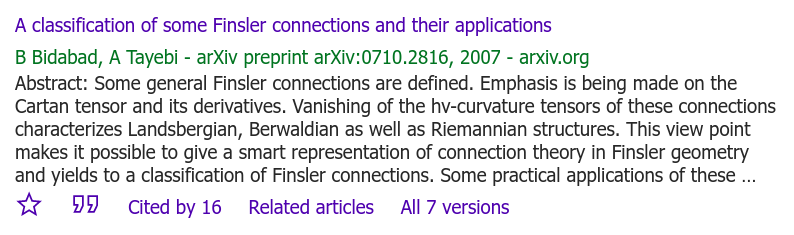
\includegraphics[height=3cm]{bidabad}
    \caption{نمونه یک مقاله در گوگل اسکولار}
    \label{fig:bidabad}
    \end{figure}
    
    پس از پیدا کردن این مقاله، مانند شکل~\ref{fig:bidabad}، در زیر نام و چکیده‌ٔ مقاله، چند گزینه وجود دارد.
    در اینجا ما به گزینه‌ٔ دوم 
    (\raisebox{-4pt}{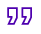
\includegraphics[scale=.4]{comma}}) احتیاج داریم. بر روی آن کلیک کرده و پنجره‌ای مانند شکل~\ref{fig. 2} باز می‌شود.

    \begin{figure}[h]
        \centering
        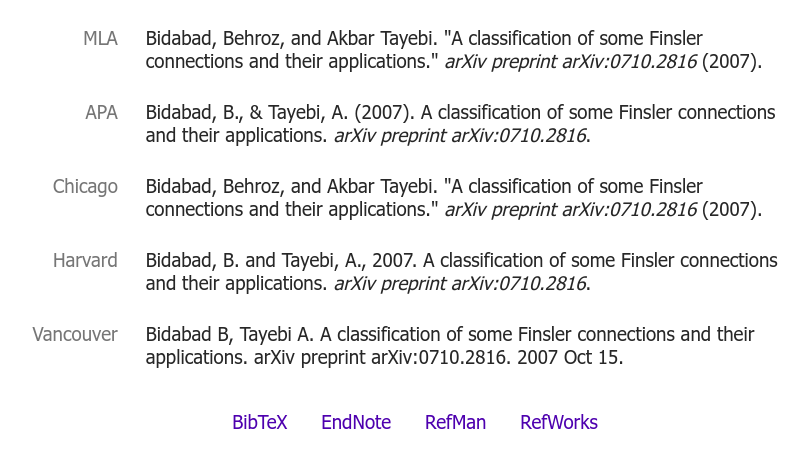
\includegraphics[width=.9\textwidth]{bibref}
        \caption{پنجره‌ٔ باز شده در گوگل اسکولار}\label{fig. 2}
    \end{figure}
    روی گزینه‌ٔ اول، یعنی    \Verb!BibTeX!    کلیک کرده و همه‌ٔ نوشته‌های پنجره‌ٔ باز شده را مانند زیر، کپی کرده و در فایل    \Verb!references.bib! 
    موجود در پوشته پروژه درج می‌کنیم. سپس کلیدهای  \Verb!Ctrl+s!    را می‌زنیم تا فایل ذخیره شود.
    \begin{latin}
    \begin{Verbatim}
@article{bidabad2007classification,
  title={A classification of some Finsler connections and their applications},
  author={Bidabad, Behroz and Tayebi, Akbar},
  journal={arXiv preprint arXiv:0710.2816},
  year={2007}
}
    \end{Verbatim}
    \end{latin}
    البته این تنها شیوه دریافت اطلاعات کتابشناختی نبوده و برای اطلاع بیشتر می‌توانید به راه‌های دیگری که در فصل ششم~\cite{razavianAmintoosiTayebi}
    معرفی شده‌اند مراجعه نمایید. 
    ممکن است در برخی موارد، عنوان نوع مدخل و یا فیلدهای آن را با حروف بزرگ مشاهده نمایید، برای مثال بجای \Verb+year={2007}+ نوشته 
    شده باشد \Verb+YEAR={2007}+؛ در همینجا باید متذکر شد که هر دوی این کاربردها برای \Verb!BibTeX! یکسان است و تفاوتی بین آن دو قائل نمی‌گردد.  
    
    \subsection{روش ارجاع در متن}
    برای ارجاع دادن به مقاله‌ٔ بالا، باید در جایی که می‌خواهید ارجاع دهید، دستور  
     \linebreak  \LR{\Verb+\cite{bidabad2007classification}+}
    را تایپ کنید.
    همانطور که مشاهده می‌کنید از کلمه‌ای که در سطر اول آدرس مقاله آمده (یعنی کلمه‌ی پس از    \Verb+@article{+)
    استفاده کرده‌ایم. پس از دستور فوق، به صورت \cite{bidabad2007classification} مرجع خواهد خورد. 
    توجه نمایید، در صورتی مراجع چاپ خواهند شد که در متن به آن‌ها ارجاع داده شده باشد. همچنین برای ارجاع چندتایی از دستور 
    \LR{\Verb+\cite{name1, name2,...}+}
    استفاده کنید که به‌صورت 
    \cite{bidabad2007classification, razavianAmintoosiTayebi, Omidali1387Lshort} ارجاع خواهند خورد.

    \subsection{روش اجرای برنامه}
    ابتدا فایل 
        {\ttfamily \jobname.tex}
    را در ادیتور تِک/لاتِک باز کرده و آن را دو بار اجرا کنید. سپس حالت اجرا را به حالت    \Verb!Bibtex!
    تغییر داده و دوباره برنامه را اجرا کنید. دو بار دیگر برنامه را در حالت     \Verb+XeLaTeX+
    اجرا کرده و نتیجه را مشاهده کنید. 
    
    \subsection{مراجع فارسی}
    برای نوشتن مراجع فارسی نیز به طریقی مشابه در همان فایل  \Verb!references.bib!  مداخل مورد نیاز خود را 
    می‌افزاییم. تنها تفاوت در اینجا اضافه‌شدن یک فیلد دیگر برای تعیین \linebreak
    زبان حروفچینی مدخل است که در اینجا مقصود زبان پارسی است. لذا  باید فیلد \linebreak
    \Verb+LANGUAGE={Persian}+ را به مداخل فارسی خود نیز بیفزاییم. 
    \begin{LTR}
\begin{Verbatim}[commandchars=+\[\]]
@article{manifold,
    title= {+rl[هندسه منیفلد]},
    author={+rl[بیدآباد, بهروز]},
    journal={+rl[دانشگاه صنعتی امیرکبیر]},
    year={1389},
    LANGUAGE={Persian}
}
\end{Verbatim}    
    \end{LTR}
    
    \subsection{حذف مداخل}
    در صورتی که بخواهید مدخلی را از فایل مراجع خود به صورت موقتی حذف نمایید لازم به حذف کل اطلاعات مدخل مورد نظر نیست بلکه تنها 
    کافی است علامت \Verb+@+ را از ابتدای نوع مدخل مورد نظر را حذف نمایید تا دیگر در فهرست منابع و مآخذ متن قرار نگیرد؛ برای نمونه 
    \Verb+@article{+ را به  \Verb+article{+ تبدیل نمایید.
    
    
    
    \section{راهنمای واژه‌نامه}

    به دلیل پیچیدگی ایجاد واژه‌نامه‌ با کمک بسته \Verb+glossaries+، از روش زیر برای نوشتن واژه‌نامه استفاده کنید --هر چند که امکان استفاده از این 
    بسته نیز برای علاقه‌مندان ممکن است--:

    ابتدا با استفاده از نرم‌افزاری مانند \lr{Excel}، واژه‌‌های خود را یک‌ بار براساس حروف الفبای فارسی و بار دیگر انگلیسی مرتب کنید. 
    سپس واژه‌های مورد مورد نظر  را با سبکی که در ادامه توضیح داده شده است در فایل‌های
    \lr{\ttfamily dicen2fa.tex} و \lr{\ttfamily dicfa2en.tex}  
    ذخیره نموده و در کنار فایل اصلی (\texttt{\jobname.tex}) قرار دهید و بقیه کار را به استایل پایان‌نامه/رساله دانشگاه قم واگذارید تا به صورت 
    خودکار این واژه‌نامه‌ها را برایتان تولید نماید. 
    
    \subsection{سبک مورد استفاده در فایل‌های واژه‌نامه}
    در این فایل‌ها، در هر سطر باید یک مدخل و ترجمه آن قرار گیرد که با علامت ''\Verb+=+`` از هم جدا شده‌اند. 
    در حالت فارسی به انگليسی ابتدای سطر با کلمه فارسی آغاز شده و سپس در ادامه آن ترجمه انگلیسی آن می‌آید و علامت ''\Verb+=+`` نیز  این دو را 
    از هم جدا می‌نماید و در حالت انگليسی به فارسی به صورت عکس عمل می‌نمایید؛ ابتدا واژه انگلسیسی و \ldots. 
    اگر استفاده از علامت  ''\Verb+=+``  را فراموش نمایید آن مدخل در واژه‌نامه شما نشان داده نخواهد شد. ضمناً وجود خطوط خالی نیز 
    بی‌تاثیر است امّا آن چیزی که به هیچوجه نباید فراموش شود این است که هر دو واژه فارسی و انگلیسی و جداکننده بین آن دو باید در یک خط قرار گیرند. 
    برای نمونه در شکل~\ref{fig:dictionaries} 
    بخشی از محتویات قابل 
    قبول این دو فایل «واژه‌نامه فارسی به انگليسی» و «واژه‌نامه انگليسی به فارسی» آمده است.  توجه داشته باشید در صورت عدم رعایت قاعده فوق مدخل شما 
    به واژه‌نامه اضافه نخواهد شد. 

\begin{figure}[h]
\begin{minipage}{.55\textwidth}
\leftline{\Verb+dicfa2en.tex+}\vspace*{1mm}
\begin{Verbatim}[commandchars=+\[\], frame=single, framesep=1mm]
+rl[طوقه]=Loop
+rl[ظرفیت]=Valency
+rl[عدم مجاورت]=Nonadjacency
+rl[فضای برداری]=Vector space
+rl[کاملاً تحویل‌پذیر]=Complete reducibility
+rl[گراف]=Graph
+rl[ماتریس جایگشتی]=Permutation matrix 
\end{Verbatim}
\end{minipage}
\hfill
\begin{minipage}{.4\textwidth}
\leftline{\Verb+dicen2fa.tex+}\vspace*{1mm}
\begin{Verbatim}[commandchars=+\[\], frame=single, framesep=1mm]
Edge=+rl[یال]
Function=+rl[تابع]
Group=+rl[گروه]
Homomorphism=+rl[همریختی]
Module=+rl[مدول]
Natural map=+rl[نگاشت طبیعی]
One to One=+rl[یک به یک]
\end{Verbatim}    
\end{minipage}
\caption{سبک مورد استفاده در فایل‌های واژه‌نامه}
\label{fig:dictionaries}
\end{figure}

    \section{نمایه}\label{Namaye}
    
    برای ایجاد نمایه در متن باید از دستور \Verb+\index+ استفاده نمود. 
    استفاده از این دستور تنها سبب ایجاد یک اندیس در نمایه به صفحه‌ای از متن که این دستور  در آن قرار دارد می‌گردد و خود کلمه در متن اصلی حروفچینی نمی‌شود. 
    لذا معمولاً در متن اصلی حالتی شبیه به زیر رخ می‌دهد:
    
    \leftline{\LR{\ldots \Verb+word\textbackslash{}index\{word\}+ \ldots}}
    به عبارت دیگر یکبار باید کلمه \Verb+word+ را تایپ نموده و بار دیگر برای نمایه‌سازی آن دستور \Verb+\index{word}+. بسیاری از کاربران 
    برای راحت‌تر نمودن نمایه‌سازی در متن ترجیح می‌دهند برای کلمات در دو حالت فارسی و لاتین دستورات زیر را در سرآمد فایل تعریف نموده و از آن‌ها استفاده 
    نمایند. 
    
\begin{Verbatim}
\newcommand{\wi}[1]{#1\index{#1}}
\newcommand{\wil}[1]{\lr{#1}\index{\lr{#1}}}
\end{Verbatim}
    
    پس از تعریف ماکروهای فوق، برای حالتی مانند قبل تنها درج \Verb+\wi{word}+ کافی است. 

    \subsection{ساخت نمایه}
    پس از اینکه کلمات مورد نظر را در متن با دستور \Verb+\index+ مشخص نمودید حال زمان آن است که تنظیمات لازم در فایل را نیز انجام دهید. 
    ابتدا باید در سرآمد سند خود بسته \Verb+makeidx+ را بارگذاری نموده و پس از آن دستور \Verb+\makeindex+ را قرار دهید. 
    و سپس در نهایت در نقطه‌ای که تمایل به درج نمایه دارید دستور \Verb+\printindex+ را بگذارید. سپس برای ایجاد نمایه از برنامه‌هایی مانند 
    \Verb+MakeIndex+ و یا \Verb+xindy+ 
    استفاده نمایید. از آنجایی که می‌خواهید با نمایه فارسی نیز داشته باشید همانطور که پیشتر نیز اشاره گردید تنها گزینه زیندی خواهد بود زیرا که آن برنامه 
    دیگر پشتیبانی درستی از پارسی نداشته و ترتیب الفبایی درستی را برای کلماتی که با گچپژ آغاز شوند رعایت نمی‌کند. حال برای اینکه نمایه ایجاد شود 
    می‌توانید با کمک زیندی را از طریق خط فرمان (ر.ک.~صفحه~\pageref{xindy})و یا ادیتوری که از طریق آن مشغول حروفچینی سند خود هستید اقدام نمایید.
    
    اکنون به نحوه تنظیمات لازم برای اعمال زیندی روی سندتان در ادیتور \lr{\TeX{}works} که به طور پیش‌فرض بهمراه \lr{\TeX{}Live}
    عرضه می‌گردد اشاره می‌شود --اگر ادیتور دیگری را به کار می‌برید به طریقی مشابه باید اعمال زیر را انجام دهید--. 


    \subsubsection{تنظیم زیندی برای \lr{\TeX{}works}}
    ابتدا از منوی \lr{Edit} گزینه \lr{Preferences} را انتخاب نمایید. پنجره‌ای مانند شکل~\ref{fig:texworks_preferences} باز می‌گردد.%
    \footnote{از آنجایی که اسناد فارسی
    همیشه باید با \Verb+XeLaTeX+ کامپایل شوند لذا پیشنهاد می‌گردد که در همینجا پیش‌فرض را در بخش \lr{Processing Tools} 
    از \Verb+pdfLaTeX+  به \Verb+XeLaTeX+ تغییر دهید.} 
    
    \begin{figure}[h]
    \centering
    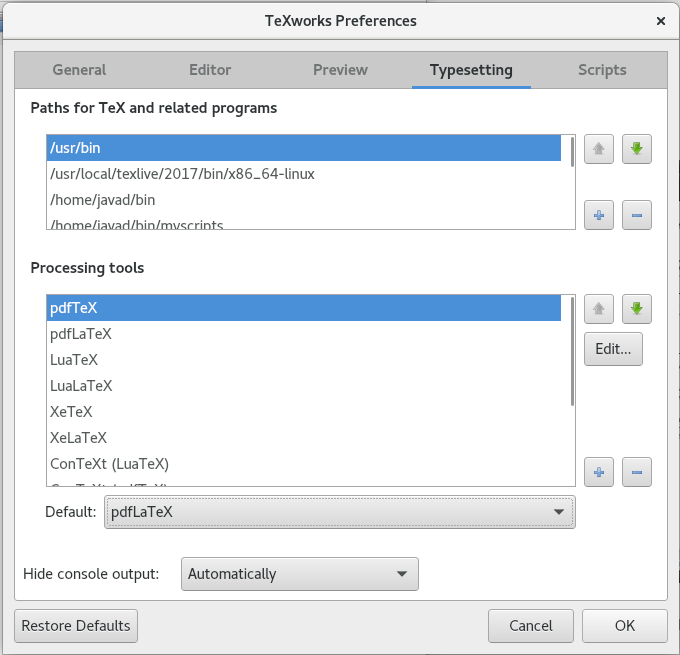
\includegraphics[width=.8\textwidth]{texworks_preferences}
    \caption{تنظیمات ابزار پردازش در تک‌ورکس}
    \label{fig:texworks_preferences}
    \end{figure}
    
    سپس دکمه علامت مثبت که در کنار جعبه  \lr{Processing Tools} قرار دارد را فشار دهید و م
    طابق با شکل~\ref{fig:texworks_xindy}
    تنظیمات لازم برای زیندی را انجام دهید. پس از انجام این گام به منوی ابزارهای پردازش گزینه \lr{XindyMakeIndex} نیز اضافه شده است که حال 
    می‌تواند آن را روی سند خود بکار بندید. 
    \begin{figure}[!h]
    \centering
    \centerline{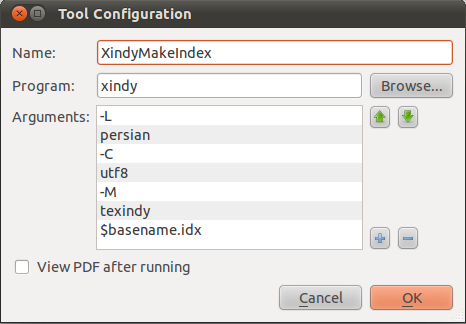
\includegraphics[width=.5\textwidth]{Xindy_Make_Index.png}}
    \caption{تنظیمات مربوط به تک‌ورکز}
    \label{fig:texworks_xindy}
    \end{figure}

    \subsection{ساخت نمایه در استایل پایان‌نامه/رساله دانشگاه قم}
    خوب شاید از توضیحات فوق خسته و شاید کمی هراسیده باشید!. لازم بذکر است 
    همانطور که جلوتر نیز اشاره گردید در استایل پایان‌نامه/رساله دانشگاه قم نیازی به هیچکدام از این کارها نمی‌باشد و تنها کاری که لازم است انجام دهید این است 
    که کلاس را با گزینه     \Verb+index+     بارگذاری نمایید:
     \LR{\Verb+\documentclass[index]{thesis-qom}+}.
     با این گزینه تمامی کارهای لازم برای ایجاد نمایه اعم از لود بسته و ساخت نمایه و پرینت آن در محل مناسب توسط خود استایل به صورت خودکار انجام خواهد شد. 
     تنها نکته‌ای که نباید فراموش نمایید این است که در این حالت برای کامپایل سند حتماً باید از سوئیچ \LR{\Verb+--shell-escape+} استفاده نمایید. 
     اگر برای کامپایل سند خود از خط فرمان استفاده می‌کند کافی است سوئیچ فوق نیز در ادامه دستورات نیز نوشته شود لکن اگر ادیتوری را بدین منظور 
     بکار می‌برید باید تنظیمات لازم برای آن را انجام دهید. برای مثال در ادیتور تک‌ورکس باید دومرتبه به بخش \lr{Preferences} مراجعه نموده و 
     گزینه زی‌لاتک را به صورتی که در تصویر~\ref{fig:texworks_shellescape} نشان داده شده است ویرایش نمایید. 
     
    \begin{figure}[!h]
    \centering
    \centerline{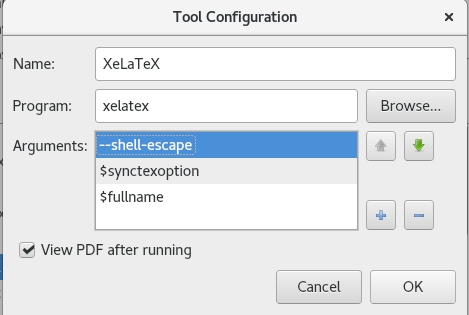
\includegraphics[width=.5\textwidth]{xindy_shellescape}}
    \caption{ تنظیمات مربوط به سوئیچ  \lr{--shell-escape} برای زی‌لاتک}
    \label{fig:texworks_shellescape}
    \end{figure}     
    
     \index{کتاب}
    \index{پارسی‌لاتک}
    \index{بی‌دی}
    \index{سوال}
    \index{عنصر}
    \index{گزینه}
    \index{ژاکت}
    \index{مرکز دانلود}
    \index{اجرا}
    \index{تک‌لایو}
    \index{ثالث}
    \index{جهان}
    \index{چهار}
    \index{حمایت}
    \index{خواهش}
    \index{دنیا}
    \index{زی‌پرشین}
    \index{ریحان}
    \index{شیرین}
    \index{صمیمی}
    \index{ضمیر}
    \index{طبیب}
    \index{آنومالی بلیدی}
    \index{همگرا}
    
 % chapter 4
%\chapter{نگارش صحیح}
%\thispagestyle{empty}
\section{مقدمه}

فصل مقدمه یک پایان‌نامه/رساله، با بیان نیاز موضوع، تعریف مسئله و اهمیت آن در یک یا چند بند (پاراگراف) آغاز می‌شود\footnote{شروع مقدمه نباید 
چنان طولانی باشد كه هدف اصلی را تحت‌ تاثیر قرار دهد.}  و با مرور پیشینه موضوع (سابقه کارهای انجام‌شده پیشین که ارتباط مستقیمی با مسئله مورد بررسی دارند) 
ادامه می‌یابد. سپس در یک یا دو بند توضیح داده می‌شود كه در این پایان‌نامه/رساله، چه دیدگاه یا راهكار جدیدی نسبت به مسئله (موضوع) مورد بررسی وجود دارد. 
به‌عبارت دیگر نوآوری‌ها به‌صورت کاملاً شفاف و صریح بیان می‌شود. در ادامه ممکن است به نتایج بدست‌آمده نیز به‌طور مختصر و کلی اشاره ‌شود. 
در آخرین بند از مقدمه به محتوای فصل‌های بعدی پایان‌نامه/رساله به‌اختصار اشاره می‌شود.

نگارش صحیح یک پایان‌نامه/رساله در فهم آسان آن بسیار موثر است. در این فصل مهمترین قواعد نگارشی که باید مورد توجه جدی نگارنده قرار گیرد، 
به اختصار بیان می‌شود. این قواعد را می‌توان در محورهای اصلی زیر دسته‌بندی کرد:

\begin{enumerate*}[label=\textbf{\alph*)}]
\item
فارسی نویسی
\item
رعایت املای صحیح 
\item
رعایت قواعد نشانه‌گذاری
\end{enumerate*}
\section{فارسی نویسی}
در حد امکان سعی کنید به جای کلمات غیر‌فارسی از معادل فارسی آن‌ها استفاده کنید، به‌ویژه در مواردی که معادل فارسی مصطلح و رایج است‌.‌ به‌طور مثال استفاده از کلمه «لذا» به‌جای «برای همین» یا «به‌همین دلیل» توجیهی ندارد‌. همچنین کلمه «پردازش» زیباتر از «پروسس» و معادل فارسی «ریز‌پردازنده» مناسب‌تر از «میکروپروسسور» است‌.‌ در این‌گونه موارد چنانچه احتمال عدم آشنایی خواننده با معادل فارسی وجود دارد، یا اصطلاح غیر‌فارسی معمول‌تر است، در اولین ظهور کلمه فارسی، اصل غیر‌فارسی آن به‌صورت پاورقی آورده شود‌.‌ اگر به‌ناچار باید کلمات انگلیسی در لابه‌لای جملات گنجانده شوند، از هر طرف یک فاصله بین آن‌ها و کلمات فارسی پیش و پس از آن‌ها در‌نظر گرفته شود‌.‌ چنانچه در پایان‌نامه/رساله از مختصر‌نویسی استفاده شود، لازم است در اولین استفاده، تفصیل آن در پاورقی آورده شود‌.‌ 

\section{رعایت املای صحیح }
رعایت املای صحیح فارسی به مطالعه و درک راحت‌تر کمک می‌کند. همچنین در نوشته‌های فارسی باید در حد امکان از همزه « ء، أ، ؤ، ة، إ، ئ» استفاده نشود‌.‌ به‌عنوان مثال «اجزاء هواپیما» و «آئین نگارش» ناصحیح، اما «اجزای هواپیما» و «آیین نگارش» صحیح هستند.‌
\section{رعایت قواعد نشانه‌گذاری}
منظور از نشانه‌گذاری به‌کار‌بردن علامت‌ها و نشانه‌هایی است که خواندن و فهم درست یک جمله را ممکن و آسان می‌کند. در ادامه نشانه‌های معمول و متداول در زبان فارسی و موارد کاربرد آن‌ها به اختصار معرفی می‌شوند.
\subsection{ویرگول}
ویرگول نشانه ضرورت یک مکث کوتاه است و در موارد زیر به‌کار می‌رود:
\begin{itemize}
\item
در میان دو کلمه که احتمال داده شود خواننده آن‌ها را با کسره اضافه بخواند، یا نبودن ویرگول موجب بروز اشتباه در خواندن جمله شود.
\item
در موردی که کلمه یا عبارتی به‌‌‌‌عنوان توضیح، در ضمن یک جمله آورده شود. مثلاً برای کنترل وضعیت فضاپیماها، به‌دلیل آن‌که در خارج از جو هستند، نمی‌توان از بالک‌های آیرودینامیکی استفاده کرد.
\item
جدا‌کردن بخش‌های مختلف یک نشانی یا یک مرجع
\item
موارد دیگر از این قبیل
\end{itemize}
پیش از ویرگول نباید فاصله گذاشته شود و پس از آن یک فاصله لازم است و بیشتر از آن صحیح نیست.
\subsection{نقطه}
نقطه نشانه پایان یک جمله است. پیش از نقطه نباید فاصله گذاشته شود و پس از آن یک فاصله لازم است و بیشتر از آن صحیح نیست.
\subsection{دونقطه}
موارد کاربرد دونقطه عبارتند از:
\begin{itemize}
\item
پیش از نقل قول مستقیم
\item
پیش از بیان تفصیل مطلبی که به اجمال به آن اشاره شده‌است.
\item
پس از واژه‌ای که معنی آن در برابرش آورده و نوشته می‌شود.
\item
پس از کلمات تفسیر‌کننده از قبیل «یعنی» و ...
\end{itemize}
پیش از دونقطه نباید فاصله گذاشته شود و پس از آن یک فاصله لازم است و بیشتر از آن صحیح نیست.
\subsection{گیومه}
موارد کاربرد گیومه عبارتند از:
\begin{itemize}
\item
وقتی که عین گفته یا نوشته کسی را در ضمن نوشته و مطلب خود می‌آوریم. 
\item
در آغاز و پایان کلمات و اصطلاحات علمی و یا هر کلمه و عبارتی که باید به‌صورت ممتاز از قسمت‌های دیگر نشان داده شود.
\item
در ذکر عنوان مقاله‌ها، رساله‌ها، اشعار، روزنامه‌ها و ...
\end{itemize}
\subsection{نشانه پرسشی}
پیش از «؟» نباید فاصله گذاشته شود و پس از آن یک فاصله لازم است و بیشتر از آن صحیح نیست.
\subsection{خط تیره}
موارد کاربرد خط تیره عبارتند از:
\begin{itemize}
\item
جدا‌کردن عبارت‌های توضیحی، بدل، عطف بیان و ...
\item
به‌جای حرف اضافه «تا» و «به» بین تاریخ‌ها، اعداد و کلمات
\end{itemize}
\subsection{پرانتز}
موارد کاربرد پرانتز عبارتند از:
\begin{itemize}
\item
به‌معنی «یا» و «یعنی» و وقتی که یک کلمه یا عبارت را برای توضیح بیشتر کلام بیاورند.
\item
وقتی که نویسنده بخواهد آگاهی‌های بیشتر (اطلاعات تکمیلی) به خواننده عرضه کند.
\item
برای ذکر مرجع در پایان مثال‌ها و شواهد.
\end{itemize}
نکته: بین کلمه یا عبارت داخل پرانتز و پرانتز باز و بسته نباید فاصله وجود داشته باشد.
\section{جدا یا سرهم نوشتن برخی کلمات}
تقریباً تمامی کلمات مرکب در زبان فارسی باید از هم جدا نوشته شوند؛ به استثنای صفات فاعلی مانند «عملگر»، «باغبان» و یا «دانشمند» و کلماتی نظیر «اینکه»، \ldots. 
در ادامه به نمونه‌هایی از مواردی که باید اجزای یک کلمه جدا، اما بدون فاصله نوشته شوند، اشاره می‌شود‌:
\begin{enumerate}
\item
در افعال مضارع و ماضی استمراری که با «می» شروع می‌شوند، لازم است که در عین جدا نوشتن، «می» از بخش بعدی فعل جدا نیافتد‌.‌ برای این منظور باید از «فاصله متصل» استفاده و «می» در اول فعل با \lr{SS}%
\footnote{\lr{Shift+Ctrl+@}؛ البته اگر از سیستم عامل لینوکس/مک و یا صفحه کلید استاندارد پارسی در ویندوز استفاده می‌کنید 
    می‌توانید از  \lr{Shift+Space} استفاده نمایید.} 
 از آن جدا شود.‌ به‌طور مثال «می‌شود» به‌جای «می شود». 
\item
	«ها»ی جمع باید از کلمه جمع بسته‌شده جدا نوشته شود. این امر در مورد کلمات غیر‌فارسی که وارد زبان فارسی شده‌اند و با حرف «ها» جمع بسته می‌شوند، مانند «کانال‌ها» یا «فرمول‌ها» مورد تاکید است.
\item
	حروف اضافه مانند «به» وقتی به‌صورت ترکیب ثابت همراه کلمه پس از خود آورده می‌شوند، بهتر است با \lr{SS} از آن جدا شوند‌.‌ مانند «به‌صورت»، «به‌عنوان» و «به‌‌‌لحاظ»‌.‌ لازم به ذکر است هنگامی که حرف اضافه «به» با کلمه پس از خود معنای قیدی داشته باشد، مثل «بشدت» یا «بسادگی»، بهتر است که به‌صورت چسبیده نوشته شود‌.
\item
	کلمات فارسی نباید با قواعد عربی جمع بسته شوند؛ پس «پیشنهادها» صحیح و «پیشنهادات» اشتباه است‌.‌
\item
	اسم‌ها و صفت‌های دو‌قسمتی مثل «خط‌چین» و «نوشته‌شده» با \lr{SS} از هم جدا می‌شود‌.‌
\item
	شناسه‌ها با \lr{SS} از کلمه اصلی جدا می‌شود‌.‌ مثل «شده‌اند»‌ و «شده‌است». 
\item
	‌ «است» هنگامی که نقش شناسه را داشته باشد توسط \lr{SS} از قسمت اصلی جدا می‌شود‌.‌ مانند «گفته‌است»‌.
\item
	بند پیشین نباید باعث افراط در استفاده از فاصله متصل شود. مثلاً عبارت «نوشته~می‌شود‌» صحیح و عبارت «نوشته‌می‌شود» ناصحیح است. 
\item
	فعل‌های دو‌کلمه‌ای که معنای اجزای آن‌ها کاملاً با معنای کل متفاوت است، بهتر است که با \lr{SS} از هم جدا ‌شوند‌.‌
\item
	کلمات مرکب مثل کلمه «دوکلمه‌ای» در عبارت «فعل‌های دوکلمه‌ای» و \linebreak  «یادداشت‌برداری».
\item
	مصدرهای دو قسمتی با \lr{SS} از هم جدا می‌شوند‌.‌ مثل «ذوب‌کردن» و «واردکردن»‌.
\item
	 صفات تفضیلی مثل « آسان‌تر».
\end{enumerate}
  % chapter 5
%\chapter{یک مثال واقعی }

\section{تانسورها}
بسیاری از تکنیک‌های هندسه به وسیله تانسور بیان می‌شوند به‌عنوان مثال متر ریمانی خودش یک تانسور است و البته تانسورها سراسر هندسه فینسلری را نیز پر کرده‌اند. به همین دلیل در اینجا قسمتی را به آن‌ها  اختصاص داده‌ایم.
\subsection{تانسورها روی یک فضای برداری}
فرض کنیم $V$ یک فضای برداری روی میدان اعداد حقیقی با بعد متناهی باشد. دقت کنید که در سراسر این پایان نامه همه‌ی فضاهای برداری با بعد متناهی هستند مگر اینکه خلافش صریحا ذکر شود و البته همه فضاهای برداری بدون استثناء روی میدان اعداد حقیقی در نظر گرفته می‌شوند. می‌دانیم که  $ V^* $، دوگان فضای $ V $، مجموعه همه یک فرمی‌ها و یا همان تابعک‌های خطی روی $V$  می‌باشد. نگاشت طبیعی 
$ V^* \times V \longrightarrow \mathbb{R} $ را اینگونه نمایش می‌دهیم
\begin{align*}
\left\lbrace
\begin{array}{lr}
V^* \times V \longrightarrow \mathbb{R} & \quad\\
\left( \omega,X\right)  \longmapsto \left \langle \omega,X \right \rangle = \omega(X) & \omega \in V^*,  \quad X \in V
\end{array}
 \right. 
\end{align*}
یک تانسور $ k $ - هموردا روی $ V $ نگاشت چند خطی 
\begin{align*}
F: \underbrace{V\times\cdots\times V}_{\text{بار}\ k} \longrightarrow \mathbb{R}
\end{align*}
 می‌باشد. به طور مشابه یک تانسور $ l $- پادوردا یک نگاشت چند خطی به صورت زیر است: 
\begin{align*}
F:\overbrace{V^*\times\cdots\times V^*}^{\text{بار}\ l}\longrightarrow \mathbb{R}
\end{align*}
اغلب اوقات ما تانسورهایی داریم که ترکیبی از این دو حالت فوق‌اند. یک تانسور $\binom{k}{l} $ که به آن $k$-هموردا و $l$-پادوردا می‌گوییم یک نگاشت چند خطی به فرم 
\begin{align*}
F:\overbrace{V^*\times\cdots\times V^*}^{\text{بار}\ l}%
\underbrace{\times V\times\cdots\times V}_{\text{بار}\ k}\longrightarrow \mathbb{R}
\end{align*}
می‌باشد. در واقع در بسیاری از حالات با نگاشت‌هایی چند خطی سروکار داریم که $l$ تا پارامتر 1-فرمی و $k$ پارامتر برداری دارند ولی ترتیب پارامترهایشان لزوما مثل فوق نیست با این حال به آن‌ها نیز تانسور نوع $\binom{k}{l}$ می‌گوییم.\\
مجموعه همه تانسورهای $k$-هموردا را با $T^k(V)$، فضای همه تانسورهای $ l $ - پادوردا را با $T_l(V)$ و همچنین مجموعه‌ی همه تانسورهای $ \binom{k}{l} $ را  با  $ T^k_l(V) $ نمایش می‌دهیم. تساوی‌های $T^k_\circ(V) = T^k(V)$، $T^\circ_l(V) = T_l(V)$، $T^1(V)=V^*$ و $T_1(V) = V^{**}$ بدیهی هستند. همین طور
 \mbox{قرار‌داد} 
  می‌کنیم که $T^\circ(V) = \mathbb{R}$. 
\subsection{ضرب تانسورها}
ضرب روی تانسورها به روش بسیار طبیعی تعریف می‌شود. اگر $F$ یک تانسور $\binom{k}{l} $ و $G$ یک تانسور $\binom{p}{q} $ باشد $F \otimes G$ به روش زیر تعریف می‌شود
\begin{align*}
&F\otimes G(\omega^1,\cdots,\omega^{l+q},X_1,\cdots,X_{k+p}) =\\ 
&\quad F(\omega^1,\cdots,\omega^l,X_1,\cdots,X_k)G(\omega^1,\cdots,\omega^q,X_1,\cdots,X_p)  
\end{align*}
و روشن است که تانسور بدست آمده یک تانسور $\binom{p+k}{q+l} $ خواهد بود.

\section{منیفلد و کلاف برداری}

\subsection{منیفلد}

فرض کنید $ M $ یک فضای توپولوژیک باشد.  $ M $ را یک منیفلد توپولوژیک $ n $ - بعدی گویند هرگاه در شرایط زیر صدق کند: \\
1. $ M $ یک فضای هاسدورف باشد؛\\
2. $ M $ شمارای نوع دوم باشد؛\\
3. $ M $  موضعا اقلیدسی $ -n $  بعدی باشد.\\
در طول این پایان نامه، منیفلدها هموار، هاوسدورف و شمارای نوع دوم در نظر گرفته می‌شوند.

\begin{definition}
زوج مرتب $(U,\phi)$ را  که $ U $ زیر  مجموعه‌ی بازی در $ M $ و 
$ \phi :U \longrightarrow \tilde{U }$
همئومورفیسمی  از  $ U $  به  زیر مجموعه‌ی  باز  
$  \tilde{U}  $  از  $ \mathbb{R}^n  $ 
باشد یک  کارت  مختصات  روی  منیفلد  $ M $  گویند.
\end{definition}

مختصات موضعی برای  یک کارت $(x,U)$ را به صورت $(x^1,\cdots,x^n)$ و یا $(x^i)$ می‌نویسیم
و هرگاه کارت متناظر $(x,U)$ برای $ TM $ مدنظر باشد $ (x^1,\cdots,x^n,y^1,\cdots,y^n) $ نشان دهنده‌ی 
بردار
 $y^{1}\frac{\partial}{\partial x^{1}}+\cdots+y^{n}\frac{\partial}{\partial x^{n}}$ در نقطه $p$ به مختصات 
موضعی $(x^1,\cdots,x^n)$ خواهد بود. والبته همین‌طور که می‌دانیم $\frac{\partial}{\partial x^i}$ یک بردار در نقطه ی $p$ است که معادل با مشتق‌گیری
\[ X.f =\frac{\partial}{\partial x^i}\bigg|_{x(p)}fox^{-1}\qquad f\in C^\infty(M)\]
در نقطه‌ی $x(p) = (x^1,\cdots,x^n)$ می‌باشد. اغلب (ولی نه همیشه) از $\partial_i$ به جای $ \frac{\partial}{\partial x^i}$ استفاده خواهیم کرد. حال با توجه به آنچه گفتیم و نمادگذاری انیشتینی  می‌توان نوشت 
\[ (x^1,x^2,\cdots,x^n,y^1,y^2,\cdots,y^n) = y^i\partial_i\]
\subsection{کلاف‌های برداری}
هنگامی که فضای مماس تمام نقاط منیفلد را به نقاط متناظرشان ملحق کنیم مجموعه‌ای بدست می‌آوریم که می‌توان هم به‌صورت مجموعه‌ای از فضاهای برداری و هم به‌عنوان یک منیفلد به آن نگاه کرد. چنین ساختارهایی در هندسه (دیفرانسیل) چنان رایجند که نام خاصی به آن‌ها اختصاص یافته است.
یک کلاف برداری (هموار) $k$-بعدی  عبارت است از دو منیفلد $E$ (منیفلد مماس) و $M$ (منیفلد پایه) به‌همراه نگاشت $\pi:E\longrightarrow M$ (نگاشت تصویر) که در شرایط زیر صدق کند\\
1) هر  
$ E_p= \pi^{-1}(p ) $ 
(به آن تار $E$ روی $p$  می‌گوییم) دارای ساختار فضای برداری باشد.\\
2) برای هر $p\in M$ همسایگی $U$ از $p$، دیفئومورفیسم 
$ \varphi:\pi^{-1}(U)\longrightarrow U\times \mathbb{R}^k $
 که به آن ساده‌ساز موضعی می‌گوییم چنان موجود باشد که نمودار زیر جابجایی شود

 $$ \begin{CD}
 \pi^{-1}U@>\varphi>>U\times\mathbf{R}^k\\
 @V\pi VV @VV{\pi}_1 V\\
 U @= U
 \end{CD} $$
 
که در آن $\pi_1$ تصویر روی مولفه‌ی اول است.\\
3) تحدید $\varphi$ به هر تار ( یعنی تابع $\varphi:E_p\longrightarrow \left\lbrace p \right \rbrace\times \mathbb{R}^k$ ) یک 
ایزومتری خطی باشد.  \\                                          
\begin{definition}
فرض  کنیم 
$ (E^*,\pi,M,F) $  یک   کلاف  برداری  باشد و  قرار دهیم:  
$$ E ^*= \cup _{p \in M} E_p ^* $$ 
    در این  صورت $  E^* $   دارای  خاصیت  کلاف  برداری است  که  نگاشت  تصویر  آن 
$$ \pi : u \in  E_p ^* \longrightarrow p \in M $$
  می‌باشد $ E ^* $ را کلاف  دوگان  $ E $   می‌نامیم.
\end{definition}

ما دو کلاف برداری بسیار آشنا را می‌شناسیم: $TM$ و $T^*M$ که تار روی $p$ در آن‌ها به 
ترتیب $ T_pM $ و 
$ T^*_p M = (T_p M)^* $
 می‌باشد.
\begin {definition}(برش)
فرض کنید $ E $ یک  کلاف برداری  روی $ M $   با  نگاشت  $ \pi $  و  $ U \subset M $ 
یک  مجموعه‌ی  باز  در $ M $ باشد.  نگاشت  هموار $ S : U \longrightarrow E $
را  یک  برش  $ E $ روی $ U $ می‌نامیم هرگاه  به ازای  هر  $ p $ عضو  
$ U $، $ S(p) \in {E_p} $ 
. $ S $ را  یک  برش  سراسری  گوییم  هرگاه $ U = M $.
 \\ اگر  $ U \subset M $  باشد، $ S $  را  یک  برش  موضعی  روی  $ U $   می‌نامیم. مجموعه  تمام  برش‌های $ M $ را  با  نماد  $ \Gamma (M , E) $ 
نشان  می‌دهیم. لذا اگر $E = TM$ آنگاه برش مذکور همان میدان برداری خواهد بود.
\end{definition}

\begin{definition}(یکریختی  کلاف  برداری)
فرض کنید 
$ (E,\pi, M) $ و $ ( E^ \prime , \pi ^ \prime , M^ \prime) $
دو کلاف  برداری  باشند.  دو تایی  $ (F ,f ) $ از نگاشت‌های  $ C ^r $، 
$ F :E \longrightarrow E^ \prime $ و  $ f : M \longrightarrow M^ \prime $
 را  یک  یکریختی  کلاف  برداری  می‌نامیم اگر  برای  هر $ m \in M $ نگاشت  خطی 
 $$ F |_{E_m}: E_m \longrightarrow E _{f(m)}^ \prime $$
 یک  یکریختی  و  $ f $  دیفئومورفیسم  باشد. آنگاه  می‌نویسیم
 $ E \cong E^ \prime  $. 
\end{definition}
\begin {definition}
فرض کنیم $ M $ یک منیفلد $ C^{\infty} $  و $ T_{x}M $ فضای مماس در نقطه $ x\in M $  باشد. کلاف مماس بر $ M $ را با عبارت $ TM:=\bigcup_{x\in M} T_{x}M $  نمایش می‌دهیم. نگاشت تصویر طبیعی عبارت است از:
\begin{equation*}
\pi:TM \rightarrow M
\end{equation*}
که در آن $ \pi(x,y)=x $. فضای دوگان $ T_{x}M $ توسط $ T^*_{x}M $ نمایش داده شده و فضای کتانژانت در نقطه $ x \in M $ نامیده می‌شود. کلاف $ T^*M:=\bigcup_{ x\in M}T^*_{x}M $ کلاف کتانژانت نام دارد.\\
\end{definition}

\subsection{کلاف برگشت }
فرض  کنیم 
$ (E,\pi,N ) $
یک  کلاف  برداری و 
$ f: M \longrightarrow N $
نگاشتی  هموار  بین دو منیفلد
$ M $ 
و 
$ N $
باشد. با استفاده از 
$ f $
 می‌توان یک  کلاف  برداری روی 
$ M $
با همان تار کلاف  برداری 
$ (E,\pi, N) $
تعریف نمود. این  ساختار جدید را کلاف برگشت  می‌نامیم و به صورت زیر تعریف  می‌کنیم.
\begin{definition}[کلاف فیبره برگشت]
فرض  می‌کنیم $ (E,\pi,N,F) $ یک کلاف تاری و $$ f:M \rightarrow N $$  یک نگاشت هموار باشد. کلاف برگشت $E $ را با نماد $ f^*E $ نشان داده و آن را به‌صورت زیر تعریف  می‌کنیم:

$$ f^*E=\{(x,v) \in M \times E \rvert f(x)=\pi (v)\} $$
که در آن نمودار زیر جابجایی است:
	$$\begin{CD}
	f^*E@>>>E\\
	@VVV @VV\pi V\\
	M @>>f>N
	\end{CD}$$
\end{definition}

\subsection{زیر کلاف}
اگر 
$ (E_1, \pi_1, M_1, F_1) $
 و 
 $ (E_2, \pi_2, M_2, F_2) $
 دو  کلاف  برداری  باشند  به‌طوری   که  $ E_2$ و $ M_2 $ و  $ F_2 $
  به‌ترتیب  زیر منیفلدهای  $ E_1 $ و  $ M_1 $ و  $ F_1 $  باشند آنگاه  $ E_2 $ را  زیر  کلاف 
   \LTRfootnote{subbundel}
   $ E _1 $
    می‌گویند،  اگر  برای  هر  کارت  کلاف  تاری   $ ( \pi_2, \psi_ 2) $
   روی  $ U_2 \subset M_2 $  در کلاف 
  $ E_2 $، 
   یک  همسایگی  $ U _1 \subset M_1 $ و  یک  کارت  کلاف  تاری   $ (\pi_1, \psi _1) $ 
   روی  $ U _1 $  در  کلاف  
  $  E _ 1 $
     وجود  داشته  باشد  به‌طوری  که  
  $$ \Big( \pi_1, \psi _1|_{\pi _1^{-1}(U_1 \cap U_2)} \Big) = \Big( \pi_2, \psi _2|_{\pi _2^{-1}(U_1 \cap U_2)} \Big) $$
\subsection{زیر کلاف‌های افقی و قائم}
%---------------------------------------------------------------------------
\begin{definition}[زیر کلاف قائم]
فرض  کنیم  $  M $ یک  منیفلد،  $ (E,p,M) $ یک  کلاف  برداری  از  رتبه  $ r $  روی  $ M $  و $ p:E \rightarrow M $  نگاشت  تصویر  کلاف  برداری  باشند.  اگر  $ e \in E $  برداری  دلخواه  باشد، در  این  صورت  قرار   می‌دهیم: 
\begin{equation*}
v_eE := ker(p_*)_e, \qquad vE= \bigcup_{e \in E} v_eE
\end{equation*}
تعریف  می‌کنیم  $ p:w \in v_eE \rightarrow e \in TM $.  در  این  صورت  $ (vTM,p,TM) $  یک  کلاف برداری از  رتبه  $ r $ است، این  کلاف  برداری  را  کلاف  قائم  می‌گوییم.
\end{definition}
\begin{definition}(زیر کلاف افقی)
فرض  کنیم $ (E,\pi,M) $  یک  کلاف  برداری  روی  $ M $  باشد. هرگاه  بتوان  $ TE $ را  به  صورت  جمع مستقیم زیر نوشت:
\begin{equation*}
TE=VE \oplus HE
\end{equation*}
که  در  آن  $ VE $ زیر کلاف عمودی است،  در  این  صورت  زیر کلاف  $ HE $  را  زیر کلاف  افقی  می‌نامیم.  با  توجه  به  جمع  مستقیم  فوق،  زیر کلاف  افقی  لزوما  یکتا  نیست.
\end{definition}

 % chapter 6

\appendix
    \chapter{راهنمای نصب  \lr{\LaTeX}} 
    \label{chap:installation}

    \section{مقدمه}
    نرم‌افزار حروفچینی \lr{\TeX} یکی از نرم‌افزارهای معروف حروفچینی متون علمی است
    که در سطح وسیعی جهت حروفچینی  مجلات و کتب استفاده می‌شود. در این متن مختصر بر آنیم
    که راهنمای سریعی برای نصب و استفاده از آن بیان کنیم با این امید که کاربران با پیگیری آن
    به راحتی  بتوانند آن را نصب و استفاده نمایند.

    قبل از این لازم است جهت واضح شدن شکل عملکرد این نرم افزار، اطلاعاتی در مورد آن داشته
    باشیم که در ادامه به آن پرداخته می‌شود.

    نرم افزار حروفچینی \lr{\TeX} یک نرم افزار مجانی است که به صورت خط فرمانی کار می‌کند، به این
    معنی که متن مورد نظر در یک فایل نوشته شده و سپس این فایل از طریق دستورات خط
    فرمان به نرم افزار حروفچین \lr{\TeX} داده می‌شود. این نرم افزار فایل داده شده را خوانده و بر
    مبنای آن متن حروفچینی شده را به صورت یک فایل (مثلا \lr{PDF}) ارائه می‌کند.

    ابزارهای پردازشی خط فرمان متعددی برای استفاده از این نرم افزار حروفچین وجود دارد که از مهمترین 
    آن‌ها می‌توان به \lr{latex}، \lr{pdflatex} و \lr{xelatex} اشاره کرد. معمولاً ما این بخش از
    نرم افزار حروفچین را موتور \lr{\TeX} می‌نامیم. این خاصیت، اولین متمایز کنندۀ این نرم‌افزار
    از سایر نرم‌افزارها نظیر \lr{Office}  است زیرا در \lr{Office} شما نتیجه نهایی را همزمان با تایپ
     می‌بینید ولی در این نرم‌افزار باید فایل را به حروفچین بدهید تا خودش شکل خروجی را آماده
     کند. عملاً به همین دلیل نیز آن را نرم‌افزار حروفچین می‌نامند، مشابه این که شما متن خام 
     خود را به یک فرد حروفچین می‌دهید تا با شکل دهی آن در قالب صفحات، آن را برای چاپ
     آماده کند.
     
     پس متن خام باید در یک ویرایشگر تایپ شده و سپس فایل حاصل (که پسوند آن \lr{.tex } است)
     به برنامۀ حروفچین
     با استفاده از خط فرمان داده شود. ویرایشگرهایی وجود دارند که امکان وارد کردن متن خام
     و به طور همزمان، امکان دادن فایل به موتور \lr{\TeX} و نشان دادن نتیجۀ حروفچینی را دارند. 
     اما تمام آن‌ها بر مبنای همان دستورات خط فرمان عمل می‌کنند و هیچکدام به تنهایی و بدون
     دسترسی به یک موتور \lr{\TeX} نمی‌توانند خروجی تولید کنند. البته هیچ وابستگی بین
     ویرایشگر و فایل تولید شده توسط آن وجود ندارد و یک فایل توسط هر کدام می‌تواند 
     تولید یا ویرایش شود یا فایل ایجاد شده توسط  یک ویرایشگر، در دیگری تغییر یابد.
     از معروف‌ترین این ویرایشگرها می‌توان به 
     \lr{WinEdit}، \lr{Texmaker}، \lr{TeXstudio}
    و  \lr{Notepad++}  اشاره کرد--اولی و آخری تنها برای سیستم عامل ویندوز موجودند. از جملهٔ ویرایشگرهایی که در دوره‌ای  میان کاربران پارسی 
    عمومیت یافت، \lr{bidiTeXmaker} بود که توسط آقای سیدرضی علوی‌زاده با افزودن مشخصه‌هایی برای کاربران پارسی‌زبان، توسعه داده شد\cite{biditexmaker}.

    \section{نصب موتور اصلی \lr{\TeX}}
    توزیع‌های مختلفی برای موتور \lr{\TeX} وجود دارد که در اینجا به نصب دو توزیع
    معروف و مجانی آن به نام‌های \lr{\TeX{}Live}  و \lr{Mik\TeX} می‌پردازیم. تاکید می‌شود که این توزیع‌ها با هم سازگار هستند، به این
    معنی که فایل آماده شده روی تمام توزیع‌های موتور \lr{\TeX} \ کار می‌کند. لذا که مهم نیست کدام
    توزیع را برای نصب انتخاب کنید.
    بسته \lr{\XePersian}  نصب می‌شود و نیاز به هیچ کار اضافی نیست. فقط لازم است
    که فونت‌های فارسی استفاده شده در متون فارسی روی سیستم~عامل نصب شده باشد. لذا
    تنها کار اضافی این است که مجموعه فونت‌های جمع آوری شده در فایل زیر روی سیستم عامل
    نصب شود. توصیه می‌شود حتی اگر فونت‌ها را روی کامپیوتر خود دارید، دوباره آن‌ها را با استفاده
    از فونت‌های فایل زیر رونویسی کنید. این کار از بسیاری مشکلات بعدی جلوگیری می‌کند.
    \begin{latin}

    \href{http://bayanbox.ir/id/4609192605141061595}{Part 1: http://bayanbox.ir/id/4609192605141061595}

    \href{http://bayanbox.ir/id/5468937351173971771}{Part 2: http://bayanbox.ir/id/5468937351173971771}

    \href{http://bayanbox.ir/id/4133277893427051503}{Part 3: http://bayanbox.ir/id/4133277893427051503}
    \end{latin}

    البته توصیه اکید پدیدآورنده بسته \lr{\XePersian} جناب دکتر وفا خلیقی  که جهت تولید متون فارسی در \lr{\TeX} 
    این بسته را ارائه کرده‌اند، استفاده از  \lr{\TeX{}Live}  است. 
    %\pagebreak
    \subsection{نصب \lr{\TeX{}Live}}
    سایت‌های معروف به \lr{CTAN}، سایت‌هایی هستند که  وظیفه توزیع نسخه‌های مختلف
    مجانی موتور \lr{\TeX} را انجام می‌دهند. با توجه به اینکه معمولاً سرعت دانلود از سایت‌های داخلی 
    بیشتر بوده و اخیرا نیز هزینه دانلود از این سایت‌ها به صورت نیم‌بها محاسبه می‌گردد لذا توصیه می‌شود به یکی از سه 
    سایتی که در ایران وجود دارد مراجعه نموده و توزیع تک‌لایو را دانلود نمایید:
    \begin{enumerate}
        \begin{LTRitems}
            \item \url{http://ctan.asis.io/}
            \item \url{http://ctan.yazd.ac.ir/}
            \item \url{http://repo.iut.ac.ir/tex-archive/}
        \end{LTRitems}
    \end{enumerate}
        امید است دیگر دانشگاه‌های ایران نیز مانند دانشگاه یزد و اصفهان اقدام به ایجاد یکی از این سایت‌ها روی سرورهای خود نمایند تا دانشجویان آن موسسات 
        بتوانند براحتی و بدون از دست دادن حجم اکانتینگ خود به مجموعه آرشیو تک دسترسی داشته باشند. 

    این سایت به صورت روزانه به روز رسانی می‌شود. می‌توان از این سایت در هر 
    لحظه آخرین نگارش‌های نرم افزارهای مربوطه را دانلود کرد. 

    برای نصب \lr{\TeX{}Live}  مراحل زیر را انجام دهید:
    \begin{enumerate}
    \item       
        ابتدا وارد یکی از سایت‌های که جلوتر اشاره شد 
     شوید و در پایین صفحه روی \lr{\TeX{}Live}
     کلیک کنید.
     \item
      روی مسیر \lr{Images} کلیک کنید و از فولدر باز شده فایل با نام 
     	\lr{texlive.iso} 
     	را دانلود کنید. دقت کنید که حجم این فایل  در حال حاضر 
	    حدود $3.4$ گیگابایت است.
     \item
      پس از دانلود کامل، آن را با نرم افزار \lr{WinRaR}  باز کنید و در  پوشه‌ای به نام \lr{TeXLive} فایل را \lr{Extract} کنید.
     \item 
     وارد این پوشه شوید و برنامه \LR{\Verb+install-tl-windows+}
     را اجرا کنید. ادامه روند مشابه نصب سایر نرم افزارها 
     است. روند نصب بسته به سرعت کامپیوتر شما ممکن است تا یک ساعت طول بکشد.

     \item
      پس از پایان نصب، موتور \lr{\TeX} آماده استفاده است. اگر قصد استفاده از \lr{\XePersian}
     \ دارید، فقط لازم است فونت‌های مربوطه را که در بالا لینک آن آمده است را نصب کنید.
    \end{enumerate}
    بهتر است بعد از نصب؛ بسته‌های این نرم افزار را با روش زیر به روز رسانی کنید.
    \subsubsection{بروزرسانی بسته‌های \lr{\TeX{}Live} }
    دقت کنید که برای بروزرسانی شما باید به اینترنت متصل باشید زیرا بروزرسانی با استفاده از اینترنت انجام می‌شود.
    \begin{enumerate}
    \item ابتدا در قسمت برنامه‌ها، برنامه \lr{\TeX{}Live manager} را اجرا کنید.
    \item 
        مسیر به روزرسانی را یکی از سایت‌های داخلی انتخاب کنید. انتخاب هر مسیر دیگر اشکالی ندارد ولی روی سرعت گرفتن فایل‌ها و هزینه اینترنت تاثیر مستقیم دارد. 
    \item 
        سپس بسته‌های مشخص شده را به روزرسانی کنید. پس از بروز رسانی این بسته‌ها، برنامه بسته می‌شود و لازم است دو مرحله قبل تکرار شود.
        البته با این روش می‌توانید تنها بسته خاصی را بروزرسانی نمایید لکن این حالت خیلی توصیه نمی‌شود زیرا بسیاری از بسته‌ها به یکدیگر وابسته هستند. 
    \item 
        حال روی \lr{Updtate all installed} کلیک کنید. به روزرسانی نیز مشابه نصب مدت زمانی که به سرعت کامپیوتر و سرعت اینترنت شما وابسته است طول می‌کشد.
    \end{enumerate}

    \subsection{نصب  \lr{Mik\TeX}}
        از آنجایی که توصیه اکید توسعه‌دهندگان زی‌پرشین بر استفاده از تک‌لایو است لذا این بخش خیلی توضیح داده نمی‌شود و تنها به همین میزان 
        اکتفا می‌گردد که می‌توانید از همان سایت‌هایی که پیشتر معرفی گردیدند میک‌تک را دانلود نمایید. تنها نکته‌ای که باید توجه داشته باشید این است 
        که میک‌تک در نسخه‌ مینیمال نیز عرضه می‌گردد لکن برای استفاده از زی‌پرشین این نسخه‌ها ناکارآمد است و باید نسخه کامل آن را نصب نمایید. 
        

    \section{نصب \lr{Notepad++}}
    ادیتور \lr{Notepad++}  به دلیل قابلیت فارسی نویسی و همچنین از راست به چپ نویسی و امکان اجرای دستورات خط فرمان در ادیتور،
    انتخاب مناسبی برای نوشتن متون  است. برای فعال کردن قابلیت اجرای دستورات خط فرمان با استفاده از کلید \lr{F6}، پس از نصب نرم افزار \lr{Notepad++ }، 
    لازم است تا پلاگین \lr{NppExec} را نصب نمایید. بدین منظور از منوی     \lr{Plugins -> Plugin Manager -> Show Plugin Manager}
    پلاگین \lr{NppExec}  را انتخاب نموده و \lr{Install} را بزنید تا پلاگین مورد نظر نصب شود. البته این ادیتور پلاگین‌های بسیار زیادی دارد 
    که قابلیت‌های خوبی را به آن می‌افزاید که می‌تواند به کمکتان آید لذا بررسی آن‌ها خالی از فایده برایتان نخواهد بود.
    اگر از این طریق قادر به نصب پلاگین مورد نظر نشدید می‌توانید با مراجعه به آدرس \url{https://sourceforge.net/projects/npp-plugins/files/NppExec/}
    آن را دانلود نموده و سپس محتویات فایل زیپ را  در پوشه \lr{Plugins} که در محل نصب \lr{Notepad++}  قرار دارد کپی نمایید. 
    حال با زدن کلید \lr{F6}  در ادیتور، پنجره اجرای دستور باز می‌شود.
    نمونه دستوری که می‌توانید وارد کنید به صورت زیر است:

\begin{latin}
    \begin{Verbatim}
    NPP_SAVE
    cd $(CURRENT_DIRECTORY)
    xelatex --shell-escape $(NAME_PART)
    \end{Verbatim}
\end{latin}    

    برای تایپ از راست به چپ کلیدهای \lr{Alt+CTRL+R}  را بزنید و برای از چپ به راست نویسی کلیدهای \lr{Alt+Ctrl+L}  را بزنید.

    برای نیم فاصله، کلید استاندارد \lr{Ctrl+SHift+2}  است که در این ادیتور به دلیل استفاده از این ترکیب برای کار دیگری عمل نمی‌کند.
    برای عمل کردن آن باید این ترکیب کلید را از ادیتور حذف کنید. برای این منظور از منوی \lr{Settings -> Shortcut Mapper}
     در برگه \lr{Main Menu}  در ردیف حدودا ۱۱۰  این ترکیب را پیدا کرده و به چیز دیگری (مثلا \lr{CTRL+Shift+T}) عوض کنید.

     پس از این کار ترکیب  \lr{Ctrl+SHift+2} برای نیم فاصله (وقتی زبان فارسی باشد) کار می‌کند.
     
     توجه: برای تهیه فایل مقاله یا کتاب با \lr{\XePersian}، باید از کد \lr{UTF8}  برای کدگذاری فایل استفاده شود. برای انتخاب در ادیتور، از منوی
     \lr{Encoding}  گزینه مورد نظر انتخاب شود.
 % appendix 1
\chapter{آنچه باید بدانید}\label{App:App1}
در این بخش با نحوه مناسب درج منابع، نمونه مثال‌هایی از جدول، نمودار و الگوریتم در لاتک  آشنا خواهیم شد.



\section{ مدیریت مراجع با \texorpdfstring{\lr{Bib\TeX}}{Bib\TeX} }
در بخش \ref{Sec:Ref} اشاره شد که با دستور  \lr{\textbackslash bibitem}
  می‌توان یک مرجع را تعریف نمود و با فرمان \lr{\textbackslash cite}
  به آن ارجاع داد. این روش برای تعداد مراجع زیاد و تغییرات آن‌ها مناسب نیست. در ادامه به صورت مختصر توضیحی در خصوص برنامه \lr{BibTeX} که همراه با توزیع‌های معروف تِک عرضه می‌شود و نحوه استفاده از آن در زی‌پرشین خواهیم داشت.
  
یکی از روش‌های قدرتمند و انعطاف‌پذیر برای نوشتن مراجع مقالات و مدیریت مراجع در لاتک، استفاده از  \lr{BibTeX} 
 است.  روش کار با  \lr{BibTeX} به‌این صورت است که مجموعهٔ همه‌ٔ مراجعی را که در پایان‌نامه/رساله استفاده کرده یا خواهیم کرد، 
در پروندهٔ جداگانه‌ای نوشته و به آن فایل در سند خودمان به صورت مناسب لینک می‌دهیم.
 کنفرانس‌ها یا مجله‌های گوناگون برای نوشتن مراجع، قالب‌ها یا قراردادهای متفاوتی دارند که به آن‌ها استایلهای مراجع گفته می‌شود.
 در این حالت به کمک ‌استایل‌های \lr{BibTeX} خواهید توانست تنها با تغییر یک پارامتر در پروندهٔ ورودی خود، مراجع را مطابق قالب موردنظر تنظیم کنید. 
 بیشتر مجلات و کنفرانس‌های معتبر یک پروندهٔ سبک (\lr{BibTeX Style}) با پسوند \lr{bst} در وب‌گاه خود می‌گذارند که برای همین منظور طراحی شده است.

به جز نوشتن مقالات این سبک‌ها کمک بسیار خوبی برای تهیهٔ مستندات علمی همچون پایان‌نامه‌هاست که فرد می‌تواند هر قسمت از کارش را که نوشت مراجع مربوطه را به بانک مراجع خود اضافه نماید. با داشتن چنین بانکی از مراجع، وی خواهد توانست به راحتی یک یا چند ارجاع به مراجع و یا یک یا چند بخش را حذف یا اضافه ‌نماید؛ 
مراجع به صورت خودکار مرتب شده و فقط مراجع ارجاع داده شده در قسمت کتاب‌نامه خواهندآمد. قالب مراجع به صورت یکدست مطابق سبک داده شده بوده و نیازی نیست که کاربر درگیر قالب‌دهی به مراجع باشد. 

در حال حاضر چندین قالب (استایل یا سبک) فارسی قابل استفاده هستند که توسط دکتر محمود امین‌طوسی آماده شده‌اند و در توزیع‌های تک‌لایو 
و میک‌تک موجود می‌باشند. 

با استفاده از استایل فوق می‌توانید به انواع مختلفی از مراجع فارسی و لاتین ارجاع دهید. به عنوان نمونه مرجع 
\cite{Omidali82phdThesis}
 یک نمونه پروژه دکترا (به فارسی) و مرجع 
\cite{Vahedi87} یک نمونه مقاله مجله فارسی است.
مرجع 
\cite{Amintoosi87afzayesh}  یک نمونه  مقاله کنفرانس فارسی و
مرجع 
\cite{Pedram80osool} یک نمونه کتاب فارسی با ذکر مترجمان و ویراستاران فارسی است. مرجع 
\cite{Khalighi07MscThesis} یک نمونه پروژه کارشناسی ارشد انگلیسی و
\cite{xepersian} هم یک نمونه متفرقه  می‌باشند.

مراجع 
\cite{Gonzalez02book,Baker02limits} 
نمونه کتاب و مقاله انگلیسی هستند.


\subsection{ نحوه استفاده از سبک‌های فارسی}


برای استفاده از بیب‌تک باید مراجع خود را در یک فایل با پسوند \lr{bib} ذخیره نمایید. یک فایل \lr{bib} در واقع یک پایگاه داده از مراجع\LTRfootnote{Bibliography Database}  شماست که هر مرجع در آن به عنوان یک رکورد از این پایگاه داده
با قالبی خاص ذخیره می‌شود. به هر رکورد یک مدخل\LTRfootnote{Entry} گفته می‌شود. یک نمونه مدخل برای معرفی کتاب \lr{Digital Image Processing} در ادامه آمده است:

\begin{Verbatim}
@BOOK{Gonzalez02image,
  AUTHOR =      {Rafael Gonzalez and Richard Woods},
  TITLE =       {Digital Image Processing},
  PUBLISHER =   {Prentice-Hall, Inc.},
  YEAR =        {2006},
  EDITION =     {3rd},
  ADDRESS =     {Upper Saddle River, NJ, USA}
}
\end{Verbatim}

در مثال فوق، \lr{@BOOK} مشخصهٔ شروع یک مدخل مربوط به یک کتاب و \lr{Gonzalez02book} برچسبی است که به‌این مرجع منتسب شده است.
 این برچسب بایستی یکتا باشد. برای آنکه فرد به راحتی بتواند برچسب مراجع خود را به خاطر بسپارد و حتی‌الامکان برچسب‌ها متفاوت با هم باشند معمولاً از قوانین خاصی به‌این منظور استفاده می‌شود. یک قانون می‌تواند فامیل نویسندهٔ اول+دو رقم سال نشر+اولین کلمهٔ عنوان اثر باشد. به \lr{AUTHOR} و $\dots$ و \lr{ADDRESS} فیلدهای این مدخل گفته می‌شود؛ که هر یک با مقادیر مربوط به مرجع مقدار گرفته‌اند. ترتیب فیلدها مهم نیست. 

انواع متنوعی از مدخل‌ها برای اقسام مختلف مراجع همچون کتاب، مقالهٔ کنفرانس و مقالهٔ ژورنال وجود دارد که برخی فیلدهای آن‌ها با هم متفاوت است. 
نام فیلدها بیانگر نوع اطلاعات آن می‌باشد. مثال‌های ذکر شده در فایل \lr{references.bib} کمک خوبی به شما خواهد بود. 
با استفاده از سبک‌های فارسی آماده شده، محتویات هر فیلد می‌تواند به فارسی نوشته شود، ترتیب مراجع و نحوهٔ چینش فیلدهای هر مرجع را سبک مورد استفاده  مشخص خواهد کرد.

برای عمل به‌این روش: 
\textbf{در فایل \lr{references.bib}
 که همراه با این پایان‌نامه/رساله هست، موارد مختلفی درج شده است، کافیست مراجع خود را جایگزین موارد مندرج در آن نمایید.}

پس از قرار دادن مراجع خود، یک بار \lr{XeLaTeX} را روی سند خود اجرا نمایید، سپس \lr{bibtex} و پس از آن دوبار \lr{XeLaTeX} را. 
در 
\lr{TeXstudio} و
\lr{TeXMaker} کلید \lr{F11} و در \lr{TeXWorks} هم گزینهٔ \lr{BibTeX} از منوی \lr{Typeset}، \lr{BibTeX} را روی سند شما اجرا می‌کنند.

برای بسیاری از مقالات لاتین حتی لازم نیست که مدخل مربوط به آنرا خودتان بنویسید. با جستجوی نام مقاله + کلمه \lr{bibtex}  در اینترنت سایتهای بسیاری همچون \lr{ACM} و \lr{ScienceDirect} را خواهید یافت که مدخل \lr{bibtex} مربوط به مقاله شما را دارند و کافیست آنرا به انتهای فایل \lr{MyReferences} اضافه کنید.

%از هر یک از سبکهای \lr{Persian-bib} می‌توانید استفاده کنید، البته اگر از سه استایل آخر استفاده می‌کنید و مایلید که مراجع شما شماره بخورند باید بسته \lr{natbib} را با گزینه \lr{numbers} فراخوانی نمایید.

\section{جدول}
رسم جدول نیز در لاتک کار سختی نیست.  جدول 
\eqref{tab:MotionModels}
مدل‌های تبدیل را نشان می‌دهد.

\begin{table}[ht]
\caption{مدلهای تبدیل.}
\label{tab:MotionModels}
\centering
\onehalfspacing
\begin{tabular}{|r|c|l|r|}
\hline نام مدل & درجه آزادی & تبدیل مختصات & توضیح \\ 
\hline انتقالی & ۲ & $\begin{aligned} x'=x+t_x \\ y'=y+t_y \end{aligned}$  &  انتقال دوبعدی\\ 
\hline اقلیدسی & ۳ & $\begin{aligned} x'=xcos\theta - ysin\theta+t_x \\ y'=xsin\theta+ycos\theta+t_y \end{aligned}$  &  انتقالی+دوران \\ 
\hline 
\end{tabular} 
\end{table}




\section{درج الگوریتم}
\subsection{الگوریتم با دستورات فارسی}
 الگوریتم 
 \eqref{alg:DLT} 
 یک الگوریتم با دستورات فارسی است.
\begin{algorithm}[t]
\onehalfspacing
\caption{الگوریتم \lr{DLT} برای تخمین ماتریس هوموگرافی.} \label{alg:DLT}
\begin{algorithmic}[1]
\REQUIRE $n\geq4$ زوج نقطهٔ متناظر در دو تصویر 
${\mathbf{x}_i\leftrightarrow\mathbf{x}'_i}$،\\
\ENSURE ماتریس هوموگرافی $H$ به نحوی‌که: 
$\mathbf{x}'_i = H \mathbf{x}_i$.
  \STATE برای هر زوج نقطهٔ متناظر
$\mathbf{x}_i\leftrightarrow\mathbf{x}'_i$ 
ماتریس $\mathbf{A}_i$ را با استفاده از رابطهٔ \ref{eq:DLT_Ah} محاسبه کنید.
  \STATE ماتریس‌های ۹ ستونی  $\mathbf{A}_i$ را در قالب یک ماتریس $\mathbf{A}$ ۹ ستونی ترکیب کنید. 
  \STATE تجزیهٔ مقادیر منفرد \lr{(SVD)}  ماتریس $\mathbf{A}$ را بدست آورید. بردار واحد متناظر با کمترین مقدار منفرد جواب $\mathbf{h}$ خواهد بود.
  \STATE  ماتریس هوموگرافی $H$ با تغییر شکل $\mathbf{h}$ حاصل خواهد شد.
\end{algorithmic}
\end{algorithm}

\subsection{الگوریتم با دستورات لاتین}
الگوریتم
 \ref{alg:RANSAC}
  یک الگوریتم با دستورات لاتین است.

\begin{algorithm}[t]
\onehalfspacing
\caption{الگوریتم \lr{RANSAC} برای تخمین ماتریس هوموگرافی.} \label{alg:RANSAC}
\begin{latin}
\begin{algorithmic}[1]
\REQUIRE $n\geq4$ putative correspondences, number of estimations, $N$, distance threshold $T_{dist}$.\\
\ENSURE Set of inliers and Homography matrix $H$.
\FOR{$k = 1$ to $N$}
  \STATE Randomly choose 4 correspondence,
  \STATE Check whether these points are colinear, if so, redo the above step
  \STATE Compute the homography $H_{curr}$ by DLT algorithm from the 4 points pairs,
  \STATE $\ldots$ % الگوریتم کامل نیست
  \ENDFOR
  \STATE Refinement: re-estimate H from all the inliers using the DLT algorithm.
\end{algorithmic}
\end{latin}
\end{algorithm}


\section{درج کد}
درج کد به زبانهای مختلف نیز به سادگی امکان‌پذیر است. برنامه 
\ref{Code:MATLAB1}
یک قطعه کد \lr{MATLAB} را نشان می‌دهد.
%\begin{figure}
%\begin{latin}
\begin{lstlisting}[language=MATLAB,breaklines=true,numbers=right, numberstyle=\footnotesize, numbersep=-10pt,  frame=single, breakatwhitespace=false,
caption={نمونه کد \lr{MATLAB}},label={Code:MATLAB1}]
% define a continuous function
f = '4*sin(2*pi*t)';
ezplot(f);
for i=1:10
    disp(i)
end
\end{lstlisting}
%\end{latin}


%\end{figure}
%\doublespacing


\section{فرمول‌های ریاضی}
تقریباً هر آنچه دانشجویان برای نوشتن فرمول‌های ریاضی لازم دارند، در کتاب 
\lr{mathmode}
آمده است. کافیست در خط فرمان دستور زیر را وارد کنید:
\begin{latin}
texdoc mathmode
\end{latin}
متن زیر یک متن شامل انواعی از اشیاء ریاضی است که با ملاحظه فایل \lr{.tex} این سند می‌توانید دستورات مربوطه را مشاهده فرمایید.

شناخته‌شده‌ترین روش تخمین ماتریس هوموگرافی الگوریتم تبدیل خطی مستقیم 
%(\lr{DLT\LTRfootnote{Direct Linear Transform}}) 
است.  فرض کنید چهار زوج نقطهٔ متناظر در دو تصویر در دست هستند،  $\mathbf{x}_i\leftrightarrow\mathbf{x}'_i$   و تبدیل با رابطهٔ
  $\mathbf{x}'_i = H\mathbf{x}_i$
  نشان داده می‌شود که در آن:
\[\mathbf{x}'_i=(x'_i,y'_i,w'_i)^\top  \]
و $H$ ماتریس تبدیل است.
رابطه زیر را برای الگوریتم  \eqref{alg:DLT} لازم دارم.
\begin{equation}\label{eq:DLT_Ah}
\left[
\begin{array}{ccc}
0^\top & -w'_i\mathbf{x}_i^\top & y'_i\mathbf{x}_i^\top \\ 
w'_i\mathbf{x}_i & 0^\top & -x'_i\mathbf{x}_i^\top \\ 
- y'_i\mathbf{x}_i^\top & x'_i\mathbf{x}_i^\top & 0^\top
\end{array} 
\right]
\left(
\begin{array}{c}
\mathbf{h}^1 \\ 
\mathbf{h}^2 \\ 
\mathbf{h}^3
\end{array} 
\right)=0
\end{equation}

\section{نمودار}

لاتک بسته‌هایی با قابلیت‌های زیاد برای رسم انواع مختلف نمودارها دارد. مانند بسته‌های \lr{Tikz} و  \lr{PSTricks}. 
توضیح اینها فراتر از این پیوست کوچک است.%
\footnote{
نمونه مثال‌هایی از بسته \lr{Tikz} را می‌توانید
 در \url{http://www.texample.net/tikz/examples/} ببینید. به دانشجویانی که قصد قرار دادن اشکالی همانند گراف در سند خود را دارند، توصیه می‌شود مثال‌هایی از سایت مذکور را ملاحظه فرمایند.}
یک نمونه نمودار رسم شده با بستهٔ 
\lr{TikZ}
 در شکل 
\ref{fig:parabola}
نشان داده شده است.
\begin{figure}[t]
\centering
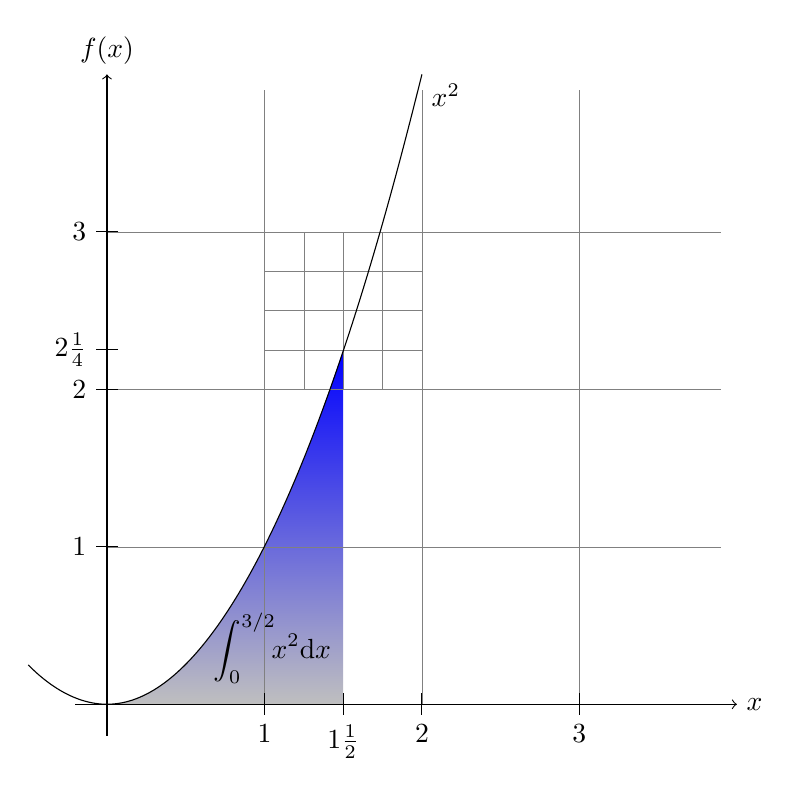
\begin{tikzpicture}[scale=2]
  \shade[top color=blue,bottom color=gray!50] 
      (0,0) parabola (1.5,2.25) |- (0,0);
  \draw (1.05cm,2pt) node[above] 
      {$\displaystyle\int_0^{3/2} \!\!x^2\mathrm{d}x$};

  \draw[style=help lines] (0,0) grid (3.9,3.9)
       [step=0.25cm]      (1,2) grid +(1,1);

  \draw[->] (-0.2,0) -- (4,0) node[right] {$x$};
  \draw[->] (0,-0.2) -- (0,4) node[above] {$f(x)$};

  \foreach \x/\xtext in {1/1, 1.5/1\frac{1}{2}, 2/2, 3/3}
    \draw[shift={(\x,0)}] (0pt,2pt) -- (0pt,-2pt) node[below] {$\xtext$};

  \foreach \y/\ytext in {1/1, 2/2, 2.25/2\frac{1}{4}, 3/3}
    \draw[shift={(0,\y)}] (2pt,0pt) -- (-2pt,0pt) node[left] {$\ytext$};

  \draw (-.5,.25) parabola bend (0,0) (2,4) node[below right] {$x^2$};
\end{tikzpicture}
\caption{یک نمودار زیبا با ارقام فارسی و قابلیت بزرگ‌نمایی بسیار، بدون از دست دادن کیفیت.}
\label{fig:parabola}
\end{figure}
موقعیت قرارگیری اشیاء شناور مانند جدول و تصویر توسط خود لاتک مدیریت می‌شود. 
گاهی موقعیت مناسب پیدا نمی‌شود و این موارد در بافر قرار می‌گیرند و در انتهای بخش یا فصل نمایش داده می‌شوند. 
برای ملزم کردن لاتک به نمایش اشیايی که در بافر دارد کافیست از دستور 
\verb!\clearpage!
استفاده کنیم.

 گاهی  ممکن است لازم باشد خودمان دستور رفتن به صفحه جدید را با دستور 
\verb!\newpage!
به لاتک بدهیم، مثل الان ...
\newpage




\section{درج توضیحات در حاشیه}
فراگیر شدن اینترنت ارتباطات از راه دور را سهل نموده است. فرض کنید دانشجو \linebreak 
پایان‌نامه/رساله خود را نوشته و از طریق اینترنت برای اظهار نظر به استاد راهنمای خود رسانده است. 
اگر قرار باشد استاد راهنما پس از مطالعه پایان‌نامه/رساله، مواردی را  گوشزد نماید، به جز راه‌های معمول (تلفن و ایمیل و ...) یک راهکار مناسب استفاده از بسته 
\lr{todonotes}
در لاتک است. به کمک این بسته که جناب آقای خلیقی از نسخه ۱۶ بسته
\lr{bidi}
امکان استفاده از آن‌را برای فارسی‌زبانان فراهم نموده‌اند، به راحتی می‌توان با استفاده از دستور
\verb!\todo{NOTE}!
نکته، یا نکات موردنظر  را در حاشیه متن یادداشت کرد.  
\todo{
توضیح بیشتری لازم است.
}

مثلاً استاد راهنما از دانشجو بخواهد که در بخشی توضیح بیشتری داده شود. استاد راهنما یا داور می‌تواند حتی محل پیشنهادی برای درج یک تصویر را به راحتی برای دانشجو مشخص کند.
\missingfigure[figwidth=\textwidth,figcolor=white]{یک تصویر از خروجی الگوریتم 
 \ref{alg:RANSAC}
را در اینجا قرار دهید.}

\todo[fancyline,color=green!30]{مرجع این مطلب؟}
بسته 
\lr{todonotes}
امکانات بسیاری دارد که با ملاحظه راهنمای آن می‌توانید با آن‌ها آشنا شوید. برای دیدن راهنما کافیست در خط فرمان دستور زیر را اجرا کنید:

\begin{latin}	
texdoc todonotes
\end{latin}	
 % appendix 2

\end{document} 
